% !TeX spellcheck = russian-aot-ieyo
% Зачем: Определяет класс документа (То, как будет выглядеть документ)
% Примечание: параметр draft помечает строки, вышедшие за границы страницы, прямоугольником, в фильной версии его нужно удалить.
\documentclass[a4paper,14pt,russian,oneside,final]{extreport}

% Зачем: Настройка Times New Roman.
% Рекомендовано для Windows (нужен PSCyr, подробности см. в fonts_windows.tex)
% раскомментировать, чтобы использовать:
% Зачем: Предоставляет проприетарный Times New Roman.
% ОБНОВЛЕНИЕ: лучше использовать scalable-cyrfonts-tex: меньше проблем с установкой
% Из руководства к PSCyr: "Во избежание проблем пакет PSCyr должен загружаться перед пакета-ми inputenc и babel".
% Примечание: Требует шаманства при установке, инструкция http://plumbum-blog.blogspot.com/2010/06/miktex-28-pscyr-04d.html
% http://blog.harrix.org/?p=444
\usepackage{pscyr}

% Зачем: Выбор внутренней TeX кодировки.
%\usepackage[T2A]{fontenc}

% не забудьте закомментировать % Зачем: Выбор внутренней TeX кодировки.
\usepackage[T2A]{fontenc}

% Зачем: Предоставляет свободный Times New Roman.
% Шрифт идёт вместе с пакетом scalable-cyrfonts-tex в Ubuntu/Debian

% пакет scalable-cyrfonts-tex может конфликтовать с texlive-fonts-extra в Ubuntu
% решение: Для себя я решил эту проблему так: пересобрал пакет scalable-cyrfonts-tex, изменив его имя. Решение топорное, но работает. Желающие могут скачать мой пакет здесь:
% https://yadi.sk/d/GW2PhDgEcJH7m
% Установка:
% dpkg -i scalable-cyrfonts-tex-shurph_4.16_all.deb

\usefont{T2A}{ftm}{m}{sl}


% Рекомендовано для Linux (нужен scalable-cyrfonts-tex, подробности см. в fonts_linux.tex)
% раскомментировать, чтобы использовать:
%% Зачем: Выбор внутренней TeX кодировки.
\usepackage[T2A]{fontenc}

% Зачем: Предоставляет свободный Times New Roman.
% Шрифт идёт вместе с пакетом scalable-cyrfonts-tex в Ubuntu/Debian

% пакет scalable-cyrfonts-tex может конфликтовать с texlive-fonts-extra в Ubuntu
% решение: Для себя я решил эту проблему так: пересобрал пакет scalable-cyrfonts-tex, изменив его имя. Решение топорное, но работает. Желающие могут скачать мой пакет здесь:
% https://yadi.sk/d/GW2PhDgEcJH7m
% Установка:
% dpkg -i scalable-cyrfonts-tex-shurph_4.16_all.deb

\usefont{T2A}{ftm}{m}{sl}
% не забудьте закомментировать % Зачем: Предоставляет проприетарный Times New Roman.
% ОБНОВЛЕНИЕ: лучше использовать scalable-cyrfonts-tex: меньше проблем с установкой
% Из руководства к PSCyr: "Во избежание проблем пакет PSCyr должен загружаться перед пакета-ми inputenc и babel".
% Примечание: Требует шаманства при установке, инструкция http://plumbum-blog.blogspot.com/2010/06/miktex-28-pscyr-04d.html
% http://blog.harrix.org/?p=444
\usepackage{pscyr}

% Зачем: Выбор внутренней TeX кодировки.
%\usepackage[T2A]{fontenc}



% Зачем: Установка кодировки исходных файлов.
\usepackage[utf8]{inputenc}

% Зачем: Делает результирующий PDF "searchable and copyable".
\usepackage{cmap}

% Зачем: Чтобы можно было использовать русские буквы в формулах, но в случае использования предупреждать об этом.
\usepackage[warn]{mathtext}

% Зачем: Учет особенностей различных языков.
\usepackage[russian]{babel}

% Зачем: Добавляет поддержу дополнительных размеров текста 8pt, 9pt, 10pt, 11pt, 12pt, 14pt, 17pt, and 20pt.
% Почему: Пункт 2.1.1 Требований по оформлению пояснительной записки.
\usepackage{extsizes}


% Зачем: Длинна, пимерно соответвующая 5 символам
% Почему: Требования содержат странное требование про отсупы в 5 символов (для немоноширинного шрифта :| )
\newlength{\fivecharsapprox}
\setlength{\fivecharsapprox}{6ex}


% Зачем: Добавляет отступы для абзацев.
% Почему: Пункт 2.1.3 Требований по оформлению пояснительной записки.
\usepackage{indentfirst}
\setlength{\parindent}{\fivecharsapprox} % Примерно соответсвует 5 символам.


% Зачем: Настраивает отступы от границ страницы.
% Почему: Пункт 2.1.2 Требований по оформлению пояснительной записки.
\usepackage[left=3cm,top=2.0cm,right=1.5cm,bottom=2.7cm]{geometry}


% Зачем: Настраивает межстрочный интервал, для размещения 40 +/- 3 строки текста на странице.
% Почему: Пункт 2.1.1 Требований по оформлению пояснительной записки.
\usepackage[nodisplayskipstretch]{setspace}
\setstretch{1.0}
%\onehalfspacing

% Зачем: Выбор шрифта по-умолчанию.
% Почему: Пункт 2.1.1 Требований по оформлению пояснительной записки.
% Примечание: В требованиях не указан, какой именно шрифт использовать. По традиции используем TNR.
\renewcommand{\rmdefault}{ftm} % Times New Roman


% Зачем: Отключает использование изменяемых межсловных пробелов.
% Почему: Так не принято делать в текстах на русском языке.
\frenchspacing


% Зачем: Сброс счетчика сносок для каждой страницы
% Примечание: в "Требованиях по оформлению пояснительной записки" не указано, как нужно делать, но в других БГУИРовских докуметах рекомендуется нумерация отдельная для каждой страницы
\usepackage{perpage}
\MakePerPage{footnote}


% Зачем: Добавляет скобку 1) к номеру сноски
% Почему: Пункты 2.9.2 и 2.9.1 Требований по оформлению пояснительной записки.
\makeatletter
\def\@makefnmark{\hbox{\@textsuperscript{\normalfont\@thefnmark)}}}
\makeatother


% Зачем: Расположение сносок внизу страницы
% Почему: Пункт 2.9.2 Требований по оформлению пояснительной записки.
\usepackage[bottom]{footmisc}


% Зачем: Переопределяем стандартную нумерацию, т.к. в отчете будут только section и т.д. в терминологии TeX
\makeatletter
\renewcommand{\thesection}{\arabic{section}}
\makeatother


% Зачем: Пункты (в терминологии требований) в терминологии TeX subsubsection должны нумероваться
% Почему: Пункт 2.2.3 Требований по оформлению пояснительной записки.
\setcounter{secnumdepth}{3}


% Зачем: Настраивает отступ между таблицей с содержанимем и словом СОДЕРЖАНИЕ
% Почему: Пункт 2.2.7 Требований по оформлению пояснительной записки.
\usepackage{tocloft}
\setlength{\cftbeforetoctitleskip}{-3em}
\setlength{\cftaftertoctitleskip}{1em}


% Зачем: Определяет отступы слева для записей в таблице содержания.
% Почему: Пункт 2.2.7 Требований по оформлению пояснительной записки.
\makeatletter
\renewcommand{\l@section}{\@dottedtocline{1}{0.5em}{1.2em}}
\renewcommand{\l@subsection}{\@dottedtocline{2}{1.7em}{2.0em}}
\makeatother


% Зачем: Работа с колонтитулами
\usepackage{fancyhdr} % пакет для установки колонтитулов
\pagestyle{fancy} % смена стиля оформления страниц


% Зачем: Нумерация страниц располагается справа снизу страницы
% Почему: Пункт 2.2.8 Требований по оформлению пояснительной записки.
\fancyhf{} % очистка текущих значений
\fancyfoot[R]{\thepage} % установка верхнего колонтитула
\renewcommand{\footrulewidth}{0pt} % убрать разделительную линию внизу страницы
\renewcommand{\headrulewidth}{0pt} % убрать разделительную линию вверху страницы
\fancypagestyle{plain}{
    \fancyhf{}
    \rfoot{\thepage}}


% Зачем: Задает стиль заголовков раздела жирным шрифтом, прописными буквами, без точки в конце
% Почему: Пункты 2.1.1, 2.2.5, 2.2.6 и ПРИЛОЖЕНИЕ Л Требований по оформлению пояснительной записки.
\makeatletter
\renewcommand\section{%
  \clearpage\@startsection {section}{1}%
    {\fivecharsapprox}%
    {-1em \@plus -1ex \@minus -.2ex}%
    {1em \@plus .2ex}%
    {\raggedright\hyphenpenalty=10000\normalfont\normalsize\MakeUppercase}}
\makeatother

% Зачем: Задает стиль заголовков подразделов
% Почему: Пункты 2.1.1, 2.2.5 и ПРИЛОЖЕНИЕ Л Требований по оформлению пояснительной записки.
\makeatletter
\renewcommand\subsection{%
  \@startsection{subsection}{2}%
    {\fivecharsapprox}%
    {-1em \@plus -1ex \@minus -.2ex}%
    {1em \@plus .2ex}%
    {\raggedright\hyphenpenalty=10000\normalfont\normalsize}}
\makeatother


% Зачем: Задает стиль заголовков пунктов
% Почему: Пункты 2.1.1, 2.2.5 и ПРИЛОЖЕНИЕ Л Требований по оформлению пояснительной записки.
\makeatletter
\renewcommand\subsubsection{
  \@startsection{subsubsection}{3}%
    {\fivecharsapprox}%
    {-1em \@plus -1ex \@minus -.2ex}%
    {\z@}%
    {\raggedright\hyphenpenalty=10000\normalfont\normalsize}}
\makeatother

% Зачем: для оформления введения и заключения, они должны быть выровнены по центру.
% Почему: Пункты 1.1.15 и 1.1.11 Требований по оформлению пояснительной записки.
\makeatletter
\newcommand\sectioncentered{%
  \clearpage\@startsection {section}{1}%
    {\z@}%
    {-1em \@plus -1ex \@minus -.2ex}%
    {1em \@plus .2ex}%
    {\centering\hyphenpenalty=10000\normalfont\normalsize\MakeUppercase}%
    }
\makeatother

% Приложения к записке
\makeatletter
\newcommand\sectionadd{%
  \clearpage\@startsection {section}{1}%
    {\z@}%
    {-1em \@plus -1ex \@minus -.2ex}%
    {1sp \@plus .1em}%
    {\centering\hyphenpenalty=10000\normalfont\normalsize\MakeUppercase}%
    }
\makeatother



% Зачем: Задает стиль библиографии
% Почему: Пункт 2.8.6 Требований по оформлению пояснительной записки.
\bibliographystyle{styles/belarus-specific-utf8gost780u}


% Зачем: Пакет для вставки картинок
% Примечание: Объяснение, зачем final - http://tex.stackexchange.com/questions/11004/why-does-the-image-not-appear
\usepackage[final]{graphicx}
\DeclareGraphicsExtensions{.pdf,.png,.jpg,.eps}


% Зачем: Директория в которой будет происходить поиск картинок
\graphicspath{{figures/}}


% Зачем: Добавление подписей к рисункам
\usepackage[nooneline]{caption}
\usepackage{subcaption}

% Зачем: чтобы работала \No в новых латехах
\DeclareRobustCommand{\No}{\ifmmode{\nfss@text{\textnumero}}\else\textnumero\fi}

% Зачем: поворот ячеек таблиц на 90 градусов
\usepackage{rotating}
\DeclareRobustCommand{\povernut}[1]{\begin{sideways}{#1}\end{sideways}}


% Зачем: когда в формулах много кириллических символов команда \text{} занимает много места
\DeclareRobustCommand{\x}[1]{\text{#1}}


% Зачем: Задание подписей, разделителя и нумерации частей рисунков
% Почему: Пункт 2.5.5 Требований по оформлению пояснительной записки.
\DeclareCaptionLabelFormat{stbfigure}{Рисунок #2}
\DeclareCaptionLabelFormat{stbtable}{Таблица #2}
\DeclareCaptionLabelSeparator{stb}{~--~}
\captionsetup{labelsep=stb}
\captionsetup[figure]{labelformat=stbfigure,justification=centering}
\captionsetup[table]{labelformat=stbtable,justification=raggedright}
\renewcommand{\thesubfigure}{\asbuk{subfigure}}

% Зачем: Окружения для оформления формул
% Почему: Пункт 2.4.7 требований по оформлению пояснительной записки и специфические требования различных кафедр
% Пример использования смотри в course_content.tex, строка 5
\usepackage{calc}
\newlength{\lengthWordWhere}
\settowidth{\lengthWordWhere}{где}
\newenvironment{explanationx}
    {%
    %%% Следующие строки определяют специфические требования разных редакций стандартов. Раскоменнтируйте нужную строку
    %% стандартный абзац, СТП-01 2010
    %\begin{itemize}[leftmargin=0cm, itemindent=\parindent + \lengthWordWhere + \labelsep, labelsep=\labelsep]
    %% без отступа, СТП-01 2013
    \begin{itemize}[leftmargin=0cm, itemindent=\lengthWordWhere + \labelsep , labelsep=\labelsep]%
    \renewcommand\labelitemi{}%
    }
    {%
    %\\[\parsep]
    \end{itemize}
    }

% Старое окружение для "где". Сохранено для совместимости
\usepackage{tabularx}

\newenvironment{explanation}
    {
    %%% Следующие строки определяют специфические требования разных редакций стандартов. Раскоменнтируйте нужные 2 строки
    %% стандартный абзац, СТП-01 2010
    \par
    \tabularx{\textwidth-\fivecharsapprox}{@{}ll@{ --- } X }
    %% без отступа, СТП-01 2013
    %\noindent
    %\tabularx{\textwidth}{@{}ll@{ --- } X }
    }
    {
    \\[\parsep]
    \endtabularx
    }


% Зачем: Удобная вёрстка многострочных формул, масштабирующийся текст в формулах, формулы в рамках и др
\usepackage{amsmath}


% Зачем: Поддержка ажурного и готического шрифтов
\usepackage{amsfonts}


% Зачем: amsfonts + несколько сотен дополнительных математических символов
\usepackage{amssymb}


% Зачем: Окружения «теорема», «лемма»
\usepackage{amsthm}


% Зачем: Производить арифметические операции во время компиляции TeX файла
\usepackage{calc}

% Зачем: Производить арифметические операции во время компиляции TeX файла
\usepackage{fp}

% Зачем: Пакет для работы с перечислениями
\usepackage{enumitem}
\makeatletter
 \AddEnumerateCounter{\asbuk}{\@asbuk}{щ)}
\makeatother


% Зачем: Устанавливает символ начала простого перечисления
% Почему: Пункт 2.3.5 Требований по оформлению пояснительной записки.
\setlist{nolistsep}


% Зачем: Устанавливает символ начала именованного перечисления
% Почему: Пункт 2.3.8 Требований по оформлению пояснительной записки.
\renewcommand{\labelenumi}{\asbuk{enumi})}
\renewcommand{\labelenumii}{\arabic{enumii})}

% Зачем: Устанавливает отступ от границы документа до символа списка, чтобы этот отступ равнялся отступу параграфа
% Почему: Пункт 2.3.5 Требований по оформлению пояснительной записки.

\setlist[itemize,0]{itemindent=\parindent + 2.2ex,leftmargin=0ex,label=--}
\setlist[enumerate,1]{itemindent=\parindent + 2.7ex,leftmargin=0ex}
\setlist[enumerate,2]{itemindent=\parindent + \parindent - 2.7ex}

% Зачем: Включение номера раздела в номер формулы. Нумерация формул внутри раздела.
\AtBeginDocument{\numberwithin{equation}{section}}

% Зачем: Включение номера раздела в номер таблицы. Нумерация таблиц внутри раздела.
\AtBeginDocument{\numberwithin{table}{section}}

% Зачем: Включение номера раздела в номер рисунка. Нумерация рисунков внутри раздела.
\AtBeginDocument{\numberwithin{figure}{section}}


% Зачем: Дополнительные возможности в форматировании таблиц
\usepackage{makecell}
\usepackage{multirow}
\usepackage{array}


% Зачем: "Умная" запятая в математических формулах. В дробных числах не добавляет пробел
% Почему: В требованиях не нашел, но в русском языке для дробных чисел используется {,} а не {.}
\usepackage{icomma}

% Зачем: макрос для печати римских чисел
\makeatletter
\newcommand{\rmnum}[1]{\romannumeral #1}
\newcommand{\Rmnum}[1]{\expandafter\@slowromancap\romannumeral #1@}
\makeatother


% Зачем: Управление выводом чисел.
\usepackage{sistyle}
\SIdecimalsign{,}

% Зачем: inline-коментирование содержимого.
\newcommand{\ignore}[2]{\hspace{0in}#2}


% Зачем: Возможность коментировать большие участки документа
\usepackage{verbatim}


\usepackage{xcolor}


% Зачем: Оформление листингов кода
% Примечание: final нужен для переопределения режима draft, в котором листинги не выводятся в документ.
\usepackage[final]{listings}


% Зачем: настройка оформления листинга для языка F#
\definecolor{bluekeywords}{rgb}{0.13,0.13,1}
\definecolor{greencomments}{rgb}{0,0.5,0}
\definecolor{turqusnumbers}{rgb}{0.17,0.57,0.69}
\definecolor{redstrings}{rgb}{0.5,0,0}

\renewcommand{\lstlistingname}{Листинг}

\lstdefinelanguage{FSharp}
    {morekeywords={abstract,and,as,assert,base,begin,class,default,delegate,do,done,downcast,downto,elif,else,end,exception,extern,false,finally,for,fun,function,global,if,in,inherit,inline,interface,internal,lazy,let,let!,match,member,module,mutable,namespace,new,not,null,of,open,or,override,private,public,rec,return,return!,select,static,struct,then,to,true,try,type,upcast,use,use!,val,void,when,while,with,yield,yield!,asr,land,lor,lsl,lsr,lxor,mod,sig,atomic,break,checked,component,const,constraint,constructor,continue,eager,event,external,fixed,functor,include,method,mixin,object,parallel,process,protected,pure,sealed,tailcall,trait,virtual,volatile},
    keywordstyle=\bfseries\color{bluekeywords},
    sensitive=false,
    morecomment=[l][\color{greencomments}]{///},
    morecomment=[l][\color{greencomments}]{//},
    morecomment=[s][\color{greencomments}]{{(*}{*)}},
    morestring=[b]",
    stringstyle=\color{redstrings},
    }

\lstdefinestyle{fsharpstyle}{
   xleftmargin=0ex,
   language=FSharp,
   basicstyle=\footnotesize\ttfamily,
   breaklines=true,
   columns=fullflexible
}

\lstdefinestyle{csharpinlinestyle} {
  language=[Sharp]C,
  morekeywords={yield,var,get,set,from,select,partial,where,async,await},
  breaklines=true,
  columns=fullflexible,
  basicstyle=\footnotesize\ttfamily
}

\lstdefinestyle{csharpstyle}{
  language=[Sharp]C,
  frame=lr,
  rulecolor=\color{blue!80!black}}


% Зачем: Нумерация листингов в пределах секции
\AtBeginDocument{\numberwithin{lstlisting}{section}}

\usepackage[normalem]{ulem}

\usepackage[final,hidelinks]{hyperref}
% Моноширинный шрифт выглядит визуально больше, чем пропорциональный шрифт, если их размеры одинаковы. Искусственно уменьшаем размер ссылок.
\renewcommand{\UrlFont}{\small\rmfamily\tt}

\usepackage[square,numbers,sort&compress]{natbib}
\setlength{\bibsep}{0em}

% Магия для подсчета разнообразных объектов в документе
\usepackage{lastpage}
\usepackage{totcount}
\regtotcounter{section}

\usepackage{etoolbox}

\newcounter{totfigures}
\newcounter{tottables}
\newcounter{totreferences}
\newcounter{totequation}

\providecommand\totfig{}
\providecommand\tottab{}
\providecommand\totref{}
\providecommand\toteq{}

\makeatletter
\AtEndDocument{%
  \addtocounter{totfigures}{\value{figure}}%
  \addtocounter{tottables}{\value{table}}%
  \addtocounter{totequation}{\value{equation}}
  \immediate\write\@mainaux{%
    \string\gdef\string\totfig{\number\value{totfigures}}%
    \string\gdef\string\tottab{\number\value{tottables}}%
    \string\gdef\string\totref{\number\value{totreferences}}%
    \string\gdef\string\toteq{\number\value{totequation}}%
  }%
}
\makeatother

\pretocmd{\section}{\addtocounter{totfigures}{\value{figure}}\setcounter{figure}{0}}{}{}
\pretocmd{\section}{\addtocounter{tottables}{\value{table}}\setcounter{table}{0}}{}{}
\pretocmd{\section}{\addtocounter{totequation}{\value{equation}}\setcounter{equation}{0}}{}{}
\pretocmd{\bibitem}{\addtocounter{totreferences}{1}}{}{}



% Для оформления таблиц не влязящих на 1 страницу
\usepackage{longtable}

% Для включения pdf документов в результирующий файл
\usepackage{pdfpages}

% Для использования знака градуса и других знаков
% http://ctan.org/pkg/gensymb
\usepackage{gensymb}

% Зачем: преобразовывать текст в верхний регистр командой MakeTextUppercase
\usepackage{textcase}

% Зачем: Переносы в словах с тире.
% Тире в словае заменяем на \hyph: аппаратно\hyphпрограммный.
% https://stackoverflow.com/questions/2193307/how-to-get-latex-to-hyphenate-a-word-that-contains-a-dash#
\def\hyph{-\penalty0\hskip0pt\relax}

% Добавляем абзацный отступ для библиографии
% https://github.com/mstyura/bsuir-diploma-latex/issues/19
\setlength\bibindent{-1.0900cm}

\makeatletter
\renewcommand\NAT@bibsetnum[1]{\settowidth\labelwidth{\@biblabel{#1}}%
   \setlength{\leftmargin}{\bibindent}\addtolength{\leftmargin}{\dimexpr\labelwidth+\labelsep\relax}%
   \setlength{\itemindent}{-\bibindent+\fivecharsapprox-0.240cm}%
   \setlength{\listparindent}{\itemindent}
\setlength{\itemsep}{\bibsep}\setlength{\parsep}{\z@}%
   \ifNAT@openbib
     \addtolength{\leftmargin}{\bibindent}%
     \setlength{\itemindent}{-\bibindent}%
     \setlength{\listparindent}{\itemindent}%
     \setlength{\parsep}{10pt}%
   \fi
}

% Нумерованный список с арабскими цифрами на всех уровнях нумерации
\newlist{legal}{enumerate}{10}
\setlist[legal]{font=\bfseries}

%\usepackage{titlesec}
%\titlespacing{\chapter}{0pt}{0pt}{4pt}

%\titleformat{\section}
    %{\normalfont\normalsize}
    %{\thesection}{1em}{\MakeUppercase}

%\titleformat{\subsection}
    %{\normalfont\normalsize}
    %{\thesubsection}{1em}{}



\newcommand{\company}{ОАО <<АГАТ -- системы управления>>}
%\newcommand{\fsharp}{F\#}
%\newcommand{\vbnet}{Visual Basic~.NET}
%\newcommand{\cpp}{C\texttt{\hspace{-0.3ex}+\hspace{-0.25ex}+}}
%\newcommand{\cppcli}{Visual \cpp{}/CLI}
%\newcommand{\dotnet}{Microsoft .NET}
%\newcommand{\netfx}{.NET Framework}
%\newcommand{\java}{Java}


\begin{document}

\begin{titlepage}
  \begin{center}
    Министерство образования Республики Беларусь \\[1em]
    Учреждение образования \\
    БЕЛОРУССКИЙ ГОСУДАРСТВЕННЫЙ УНИВЕРСИТЕТ \\
    ИНФОРМАТИКИ И РАДИОЭЛЕКТРОНИКИ \\[1em]

    Факультет компьютерных систем и сетей \\ [1em]
    Кафедра электронных вычислительных машин \\[2em]

    \begin{flushright}
      \begin{minipage}{0.4\textwidth}
        К ЗАЩИТЕ ДОПУСТИТЬ: \\
        Зав. каф. ЭВМ \\
        \underline{\hspace*{2.8cm}} Д.И.~Самаль
      \end{minipage}\\[2.2em]
    \end{flushright}

    %%
    %% ВНИМАНИЕ: на некторых факультетах (ФКП) и кафедрах (ПИКС) слова "ПОЯСНИТЕЛЬНАЯ ЗАПИСКА" предлагается (требуется) оформлять полужирным начертанием. Раскомментируйте нужную для вас строку:
    %%
    %\textbf{ПОЯСНИТЕЛЬНАЯ ЗАПИСКА}\\
    {ПОЯСНИТЕЛЬНАЯ ЗАПИСКА}\\
    {к дипломному проекту}\\
    {на тему}\\
    {СИСТЕМА ФУНКЦИОНАЛЬНОГО КОНТРОЛЯ ТЕХНИЧЕСКИХ СРЕДСТВ КОМПЛЕКСА МАШИН УПРАВЛЕНИЯ АРТИЛЛЕРИЙСКОГО ДИВИЗИОНА}\\[2em]


    {БГУИР ДП 1--40 02 01 01 065 ПЗ}\\[2em]

	  \begin{tabular}{>{\raggedright}p{0.65\textwidth}p{0.25\textwidth} }
      Студент & А.В.~Стаховский\\[1em]
      Руководитель & Т.В.~Державская \\[1em]
      Консультанты: &\\[1em]
      \hspace*{3ex}от кафедры ЭВМ & С.А.~Байрак \\[1em]
      \hspace*{3ex}по экономической части & Т.Л.~Слюсарь \\[1em]
      Нормоконтролер & А.С.~Сидорович\\[1em]
      Рецензент &
    \end{tabular}

    \vfill
    {\normalsize МИНСК 2018}
  \end{center}
\end{titlepage}
 % page 1

\sectioncentered*{Реферат}
\thispagestyle{empty}

Дипломный проект представлен следующим образом. Электронные
носители: 1 компакт-диск. Чертежный материал: 6 листов формата А1.
Пояснительная записка: \pageref*{LastPage} страниц, \totfig{}~рисунков, \tottab{}~таблицы, \totref{}~
литературных источников, 4 приложения.

Ключевые слова: функциональный контроль, техническое средство,\break АРМ, БИНС, КМУ, метеостанция, радиостанция, принтер, артиллерийский дивизион.

Целью дипломного проекта является разработка удобного в использовании инструмента, для тестирования и настройки
технических средств и локальной вычислительной сети комплекса машин управления артиллерийского дивизиона.

При разработке дипломного проекта были использованы: библиотека Qt, библиотеки протоколов и программы имитаторы, разработанные в
компании~\company.

Разработанный проект ориентирован на использование в составе комплекса автоматизации комплекса машин управления
артиллерийского дивизиона.

В разделе технико-экономического обоснования был произведен расчет затрат на создание ПО, а также прибыли от разработки,
получаемой компанией.
Проведенные расчеты показали экономическую целесообразность проекта.

Дипломный проект является завершенным. Задача, поставленная в
начале разработки, решена в полном объеме. Присутствует возможность
дальнейшего расширения и развития модуля, а также увеличение
предоставляемого функционала.

\clearpage
 %

\pagenumbering{gobble}

{
	\newgeometry{top=2cm,bottom=2.7cm,right=1.5cm,left=3cm,twoside}
  \thispagestyle{empty}
    \setlength{\parindent}{0em}

    \newcommand{\lineunderscore}{\uline{\hspace*{\fill}}}
    \newcommand\tab[1][1cm]{\hspace*{#1}}

    \begin{center}
	    Министерство образования Республики Беларусь\\[1em]
	    Учреждение образования\\
	    БЕЛОРУССКИЙ ГОСУДАРСТВЕННЫЙ УНИВЕРСИТЕТ \\
	    ИНФОРМАТИКИ И РАДИОЭЛЕКТРОНИКИ\\[1em]
    \end{center}

    \begin{minipage}{\textwidth}
	    %\begin{flushleft}
		    Факультет: КСиС. Кафедра: ЭВМ. \\
		    Специальность: 40 02 01 <<Вычислительные машины, системы и сети>>.\\
		    Специализация: 400201-01 <<Проектирование и применение локальных\break компьютерных сетей>>.
	    %\end{flushleft}
    \end{minipage}\\[1em]

    \begin{minipage}{\textwidth}
	    \begin{flushright}
		    \begin{tabular}{p{0.40\textwidth}}
			    УТВЕРЖДАЮ \\
			    Заведующий кафедрой ЭВМ \\
			    \underline{\hspace*{5em}}Д.И.~Самаль \\
			    <<\underline{\hspace*{4ex}}>>\underline{\hspace*{6em}}2018 г.
		    \end{tabular}
	    \end{flushright}
    \end{minipage}

    \begin{center}
	    ЗАДАНИЕ \\
	    по дипломному проекту студента \\
	    Стаховского Антона Владимировича
    \end{center}

    %\begin{flushleft}
	    \begin{legal}[leftmargin=*,label={\arabic*}]
	    \item Тема проекта: <<Система функционального контроля комплекса машин управления артиллерийского дивизиона>> --
		    утверждена приказом по университету от 6 апреля 2018 г. \No{601}-с.

		    \vspace{1em}

	    \item Срок сдачи студентом законченного проекта: 1 июня 2018 г.

		    \vspace{1em}

	    \item Исходные данные к проекту:

		    \begin{legal}[label*={.\arabic*}]
		    \item Операционная система: CentOS 6.
		    \item Языки программирования: C++.
		    \item Фреймворки: Qt 4.8
		    \item Система управления базами данных: PostgreSql
		    \item Среда разработки: Visual Studio 2010.
		    \end{legal}

		    \vspace{1em}

	    \item Содержание пояснительной записки (перечень подлежащих разработке вопросов):

		    Введение.
		    1. Обзор литературы.
		    2. Системное проектирование.
		    3. Функциональное проектирование.
		    4. Разработка программных модулей.
		    5. Программа и методика испытаний.
		    6. Руководство пользователя.
		    7. Экономическая часть.
		    Заключение.
		    Список использованных источников.
		    Приложения.

		    \vspace{1em}

			    \clearpage
			    \thispagestyle{empty}
	    \item Перечень графического материала (с точным указанием обязательных чертежей):
		    \begin{legal}[label*={.\arabic*}]
		    \item Вводный плакат. Плакат
		    \item Система функционального контроля технических средств КМУ артиллерийского дивизиона. Схема структурная.
		    \item Система функционального контроля технических средств КМУ артиллерийского дивизиона. Схема программы.
		    \item Система функционального контроля технических средств КМУ артиллерийского дивизиона. Диаграмма последовательности.
		    \item Система функционального контроля технических средств КМУ артиллерийского дивизиона. Диаграмма классов.
		    \item Система функционального контроля технических средств КМУ артиллерийского дивизиона. Схема адресации.
		    \end{legal}

		    \vspace{1em}

	    \item Содержание задания по экономической части: <<Технико-экономическое обоснование разработки системы
		    функционального контроля технических средств комплекса машин управления артиллерийского дивизиона>>.

	    \end{legal}
	    \vspace{1em}


	\vfill
    ЗАДАНИЕ ВЫДАЛ \hfill{} Т.Л.~Слюсарь \\

    \begin{center}
	    КАЛЕНДАРНЫЙ ПЛАН
    \end{center}

    \begin{table}[!htb]
	    \begin{tabular}{
			    | >{\raggedright}m{0.47\textwidth}
		    | >{\centering}m{0.08\textwidth}
		    | >{\centering}m{0.18\textwidth}
		    | >{\centering\arraybackslash}m{0.165\textwidth}|}
	    \hline \multicolumn{1}{|>{\centering}m{0.47\textwidth}|}{Наименование этапов\break дипломного проекта} & Объем этапа, \% & Срок выполнения этапа & Примечания \\
		    \hline Подбор и изучение литературы & 10 & 23.03--30.03 & \\
		    \hline Структурное проектирование & 10 & 31.03--06.03 & \\
		    \hline Функциональное проектирование & 20 & 07.04--20.04 & \\
		    \hline Разработка программных модулей & 30 & 21.04--01.05 & \\
		    \hline Программа и методика испытаний & 10 & 02.04--10.05 & \\
		    \hline Расчет экономической эффективности & 10 & 11.05--17.05 & \\
		    \hline Оформление пояснительной записки & 10 & 18.05--01.06 & \\
		    \hline
	    \end{tabular}
    \end{table}

	    Дата выдачи задания: 23 марта 2018 г.\\[1em]
	    Руководитель \hfill{} Т.В.~Державская \\[1em]
	    ЗАДАНИЕ ПРИНЯЛ К ИСПОЛНЕНИЮ \tab \uline{\hspace*{4em}}

	    \clearpage

	     \restoregeometry
	    }
 % pages 2 and 3. printed separately

% Зачем: Содержание пишется нормальным шрифтом, по центру всеми заглавными буквами
% Почему: Пункт 2.2.7 Требований по оформлению пояснительной записки.
%\renewcommand \contentsname {\centerline{{\normalsize{\normalfont{СОДЕРЖАНИЕ}}}}}

\renewcommand\contentsname{\hfill СОДЕРЖАНИЕ \hfill}
\renewcommand\cfttoctitlefont{\normalfont\normalsize}% use "\bfseries" if you want it in bold
\renewcommand{\cftaftertoctitle}{\hfil}

\def\formatsection{\MakeUppercase}

\makeatletter
\let\oldcontentsline\contentsline
\def\contentsline#1#2{%
  \expandafter\ifx\csname l@#1\endcsname\l@section
    \expandafter\@firstoftwo
  \else
    \expandafter\@secondoftwo
  \fi
  {%
    \oldcontentsline{#1}{\MakeTextUppercase{#2}}%
  }{%
    \oldcontentsline{#1}{#2}%
  }%
}
\makeatother

%% Зачем: Не захламлять основной файл
%% Примечание: \small\selectfont злостный хак, чтобы уменьшить размер шрифта в ToC
{
\normalfont
\tableofcontents
\newpage
}


\pagenumbering{arabic}
\setcounter{page}{7}

\sectioncentered*{Введение}
\addcontentsline{toc}{section}{Введение}
\label{sec:intro}

Защита своих границ и граждан -- одна из наиболее приоритетных задач любого государства.
Страна, которая не уделяет достаточного внимания состоянию своих войск и вооружения не может гарантировать безопасность своих граждан и сохранение дальнейшее сохранение суверенитета.

За последние десятилетия военная техника и вооружение ушли далеко вперед.
Стали широко применяться различные датчики, спутниковые системы навигации, компьютерные сети, портативные компьютеры.
Благодаря внедрению автоматизации в расчеты, настройку оборудования, тестирование периферийных устройств эффективность вооруженных сил значительно возросла.
Во время эксплуатации военной техники внезапный отказ технических средств и локальной вычислительной сети может привести
к серьезным потерям личного состава, порче оборудования, потере преимущества на местности.
В таких условиях автоматизация процессов проведения тестирования является одной из наиболее приоритетных задач.

Исключительную важность во время проведения боевых действий\break представляет комплекс машин управления огнем, который служит для управления офицерским составом деятельностью своих подчиненных.

Целью данного дипломного проекта является разработка и реализация системы автоматизации процессов тестирования технических средств и каналов обмена данными в локальной сети.
Данная система в первую очередь ориентированна на использование артиллерийским дивизионом, но при небольших доработках программные модули могут быть также использованы в решениях для других армейских подразделений.

Для успешного выполнения поставленной цели, работа над проектом была разбита на следующие задачи:
\begin{itemize}
    \item выбор технологий, удовлетворяющих требованиям;
    \item разработка управляющего модуля;
    \item разработка алгоритмов функционального контроля навигационной системы;
    \item разработка алгоритмов функционального контроля метеостанции;
    \item разработка алгоритмов функционального контроля радиостанции;
    \item разработка алгоритмов функционального контроля прибора наблюдения разведчика <<Капонир>>;
    \item разработка алгоритмов функционального контроля лазерного \break целеуказателя-дальномера;
    \item разработка алгоритмов функционального контроля принтера;
    \item разработка алгоритмов журналирования результатов тестирования;
    \item разработка программы для просмотра журнала тестирования.
\end{itemize}

Система состоит из нескольких слабо связанных модулей.
\clearpage


\section{Обзор литературы}
\label{sec:lit_review}

\subsection{Обзор существующих аналогов}
\label{sub:lit_review:analogues}
Разработанная в ходе дипломного проектировани система функционального контроля технических средств не имеет широко
известных прямых аналогов. Отсутсвие конкурирующих систем вызвано тем следующими причинами:
\begin{itemize}
	\item технические средства, предназначенные для нужд армии имеют ограниченное распространение
	\item протоколы обмена данными между техническими средствами и ЭВМ зачастую являются закрытыми
	\item модуль функционального контроля зачастую является частью закрытого проприетарного ПО, используемого для
		автоматизации задач личного состава
	\item разнообразие устройств, протоколов обмена
\end{itemize}

Таким образом, ввиду невозможности поиска аналогов среди ПО для вооруженных сил, в данном разделе будут проанализированы
наиболее близкие аналоги из других областей.

Наиболее приближенным аналогом является система функционального применяемая на железных дорогах Российской федерации
~\cite{rus_rails}.

\begin{figure}[ht]
	\centering
	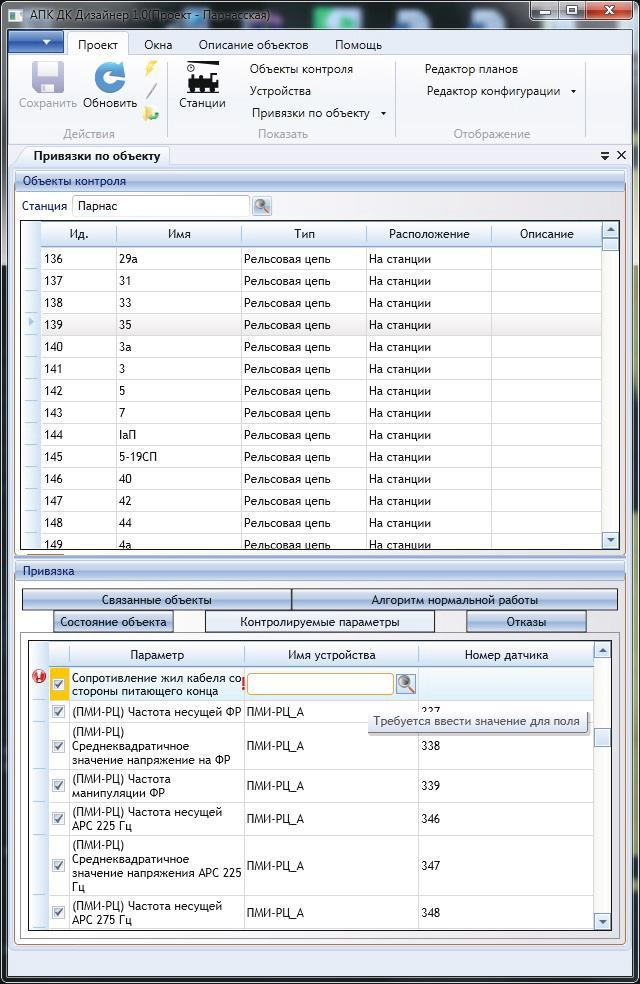
\includegraphics[scale=0.36]{rw_control}
	\caption{Модуль функционального контроля системы автоматизации РЖД~\cite{rus_rails}}
	\label{fig:lit_reiview:analogues:rw_control}
\end{figure}

Данная система функционального контроля позволяет проводить мониторинг различных учатстков железной дороги, оказывать
управляющие воздействия на объекты контроля, выводить информацию на экран или бумажный носитель, экспортировать данные в
другие программы для работы с результатами мониторинга.

Основные достоинства программы:
\begin{itemize}
	\item удобный интерфейс(использована аналогия с действующими устройствами ввода-вывода информации в
		железнодорожной автоматике и телемеханике(ЖАТ))
	\item вывод информации в иерахическом виде
	\item возможность вывода разного набора информации пользователям в зависимости от должности владельца ПК
\end{itemize}

К недостаткам можно отнести закрытость ПО, отсутствие кроссплатформенности(поддерживается только ОС Windows).

Еще один аналог -- система функционального контроля электронной аппаратуры AX518~\cite{AX518}. Система предназначена для тестирования полупроводниковых микросхем, процессоров, ЦАП, АЦП, устройств в системе радио-идентификации, устройств поддерживающих технологии широкополосного вещания и беспроводных сетей, приемопередатчиков.
Имеется возможность для проведения измерений, как в частотной, так и во временной области, спектрального анализа, измерения RF мощностей, потерь, и шумов.

Система для автоматического тестирования электронных устройств AX518 состоит из 5-слотового шасси стандарта AXIe и 18-слотового шасси стандарта PXI.
Система дополняется компьютером и программным обеспечением.
В состав программного обеспечения входят стандартные библиотеки и специфические программы для тестирования определенных устройств.

Недостатком данной системы является то, что она является аппаратно-программной. Это затрудняет ее внедрение и
значительно повышает стоимость системы.

\begin{figure}[ht]
	\centering
	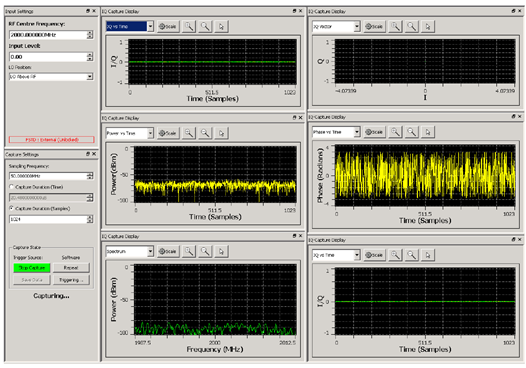
\includegraphics[scale=1.0]{ax518_soft}
	\caption{Программный модуль системы AX518~\cite{AX518}}
	\label{fig:lit_reiview:analogues:ax518_soft}
\end{figure}

\subsection{Аналитический обзор}
\label{sub:lit_review:analitics}
Технические средства(ТС) --  изделия, оборудование, аппаратура и их составные части, функционирующие на основании законов электротехники, радиотехники и электроники и содержащие электронные компоненты и схемы.

КМУ -- комплекс машин управления.
В состав комплекса машин управления огнем входят:
\begin{itemize}
	\item машина управления командира дивизиона~\cite{div_car}
	\item командно-штабная машина дивизиона
	\item машина управления командира батареи
	\item машина управления старшего офицера батареи
\end{itemize}

\begin{figure}[ht]
	\centering
	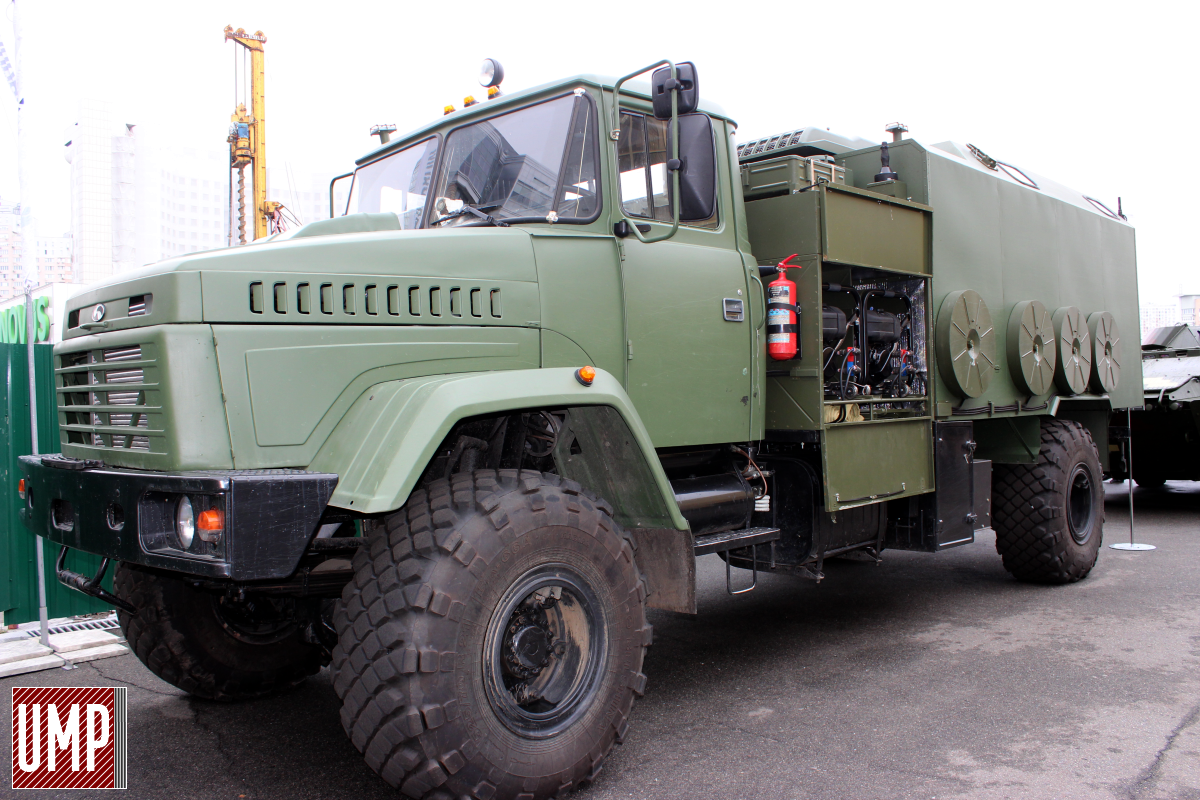
\includegraphics[scale=0.33]{div_com}
	\caption{Машина начальника штаба дивизиона на колесном шасси~\cite{div_car}}
	\label{fig:lit_reiview:analytics:div_com}
\end{figure}
В одном дивизионе имеется несколько машин разного уровня управления, содержащих в своем составе разные ТС.
Например, метеокомплект стоит только на нескольких машинах, радиостанции имеются в каждой машине, бесплатформенная
инерциальная навигационная система(БИНС) присутствует также на каждой машине, но имеют разные типы устройства, локальная вычислительная сеть(ЛВС) присутствует в каждой машине.
Программное обеспечение написано для всех машин КМУ с возможностью выборки подключенных ТС.

Разработанное в ходе дипломного проектирования программное обеспечение предназначено для развертывания в подвижном
комплексе средств автоматизации управления~\cite{patent_2263960}.
Этот подвижный комплекс средств автоматизации управления, размещенный в подвижном объекте на шасси автомобиля повышенной
грузоподъемности, содержит несколько автоматизированных рабочих места(АРМ) должностных лиц, размещенных в кузове-фургоне
подвижного объекта, оборудованных средствами вычислительной техники и средствами передачи данных, радиорелейную станцию
с антеннами, коротковолновую (KB) радиостанцию, две ультракоротковолновые (УКВ) радиостанции, локальную вычислительную
сеть (ЛВС), специальный принтер.

\begin{figure}[ht]
	\centering
	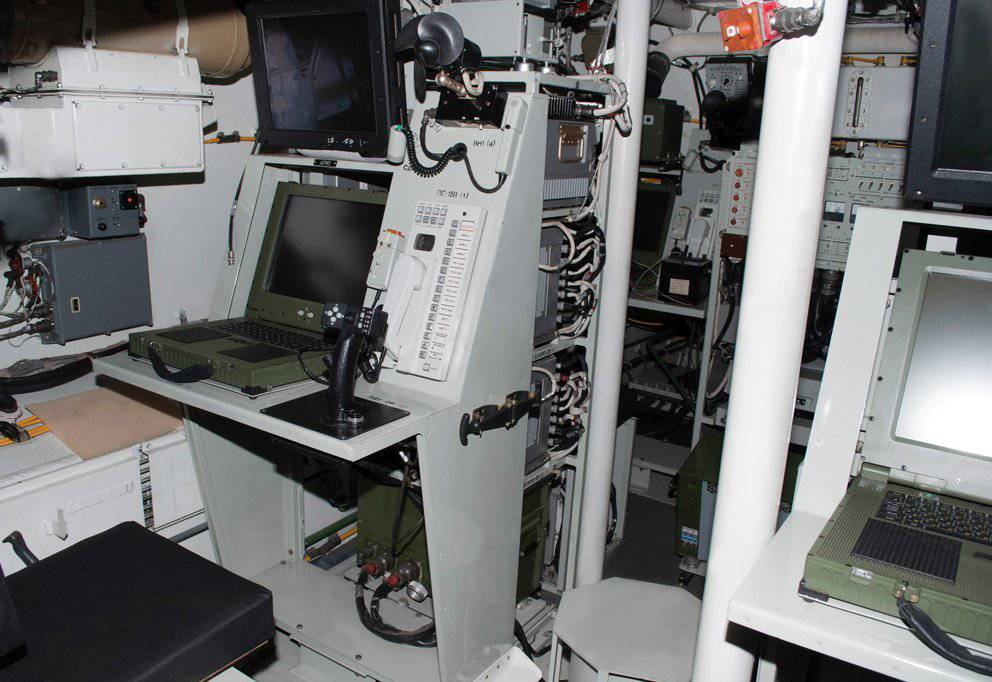
\includegraphics[scale=0.40]{arm}
	\caption{Автоматизированное рабочее место~\cite{patent_2263960}}
	\label{fig:lit_reiview:analytics:arm}
\end{figure}

Программа функционального контроля предназначена для осуществления автоматизации процессов проведения тестирования
технических\break средств.
Программа функционального контроля обеспечивает выполнение следующих функций:
\begin{enumerate}
\item тестирование средств автоматизации, локальной вычислительной сети(ЛВС), визуализацию информации о доступных в ЛВС автоматизированных рабочих местах(АРМ);
\item тестирование и настройку средств связи;
\item тестирование и настройку средств измерения.
\end{enumerate}

\subsection{Интегрированный навигационно-информационный комплекс}
\label{sub:lit_review:ins}

Интегрированный навигационно-информационный комплекс это комплексная бесплатформенная система ориентации и навигации,
построенная с использованием высокоточных акселерометров и волоконно-оптических гироскопов с замкнутым контуром,
построена на принципе комплексирования данных бесплатформенной инерциальной системы (БИНС~\cite{bins500}) с одометром, приемником спутниковых навигационных сигналов (СНС)\break GPS/GLONASS и приемником барометрического давления.
ИНИК имеет модульную систему, которая позволяет получить различные варианты системы, наиболее полно удовлетворяющие потребности по точности измерений, удобству размещения на объекте.

\begin{figure}[ht]
	\centering
	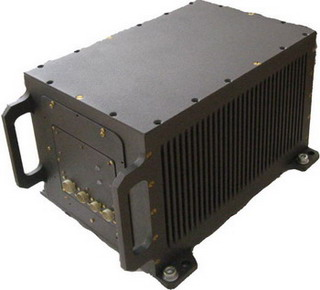
\includegraphics[scale=1.0]{bins}
	\caption{Бесплатформенная инерциальная навигационная система БИНС-500НС~\cite{bins500}}
	\label{fig:lit_reiview:ins:bins}
\end{figure}

Аппаратура позволяет  решать весь комплекс задач топопривязки, навигации и ориентирования средств ракетных войск и артиллерии в любое время в любых погодных условиях независимо от доступности сигналов СНС:
\begin{itemize}
	\item определение текущих координат объекта на стоянке (огневой позиции, районе сосредоточения), в ходе совершения марша
	\item определение углов ориентации подвижных объектов (азимутального угла продольной оси машины, углов крена и тангажа)
	\item автоматическое определения по сигналам спутниковых навигационных систем (далее СНС) GPS/GLONASS текущего единого и местного времени с использованием поправок на часовой пояс
	\item отображение на мониторе бортовой ЭВМ, индикаторных панелях текущих значений координат и высоты, а также скорости, угла продольной оси машины
	\item отображение на мониторе бортовой ЭВМ навигационной и топогеодезической информации на электронных картах местности собственного местоположения
\end{itemize}

Состав интегрированного навигационно-информационного комплекса:
\begin{itemize}
	\item блок спутниковый навигационный (БСН) с цифровым датчиком атмосферного давления
	\item цифровой одометрический датчик пути
	\item блок управления и обработки данных
	\item блок инерциальный навигационный измерительный на основе высокоточных акселерометров и волоконно-оптических гироскопов
\end{itemize}

\subsection{Многофункциональная программно-определяемая радиостанция}
\label{sub:lit_review:radio}

Радиостанции предназначены для обеспечения передачи открытой и защищеннойинформации (речевых сообщений и данных) с
повышенной помехозащищенностью и скрытностью~\cite{prc9661}.
В каждой машине КМС установлено несколько радиостанций различных типов.

Применение радиостанций:
\begin{itemize}
	\item тактическое звено управления вооруженных Сил
	\item использование в танках, БМП, БТР, автомобилях
	\item оснащение воинских подразделений наблюдения и разведки, должностных лиц уровней командования батальонами (дивизионами), ротами (батареями) и взводами
	\item оснащение командных пунктов вооруженных сил пунктов управления и узлов связи рот, батальонов и бригад
\end{itemize}

\begin{figure}[ht]
	\centering
	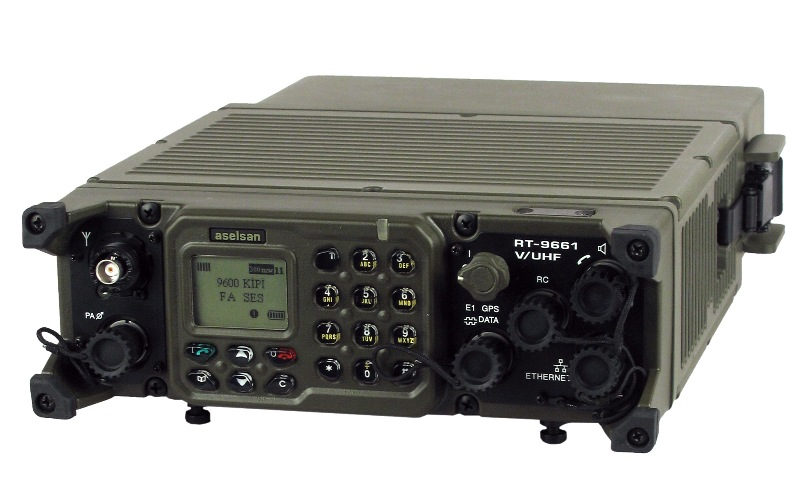
\includegraphics[scale=0.63]{radio_station}
	\caption{Радиостанция PRC-9661/VRC-9661}
	\label{fig:lit_reiview:meteo:radio_station}
\end{figure}

\subsection{Автоматическая метеостанция}
\label{sub:lit_review:meteo}

Автоматическая метеостанция(АМС) это комплексный универсальный метеорологический модуль - компактное и легкое
устройство, оснащенное набором датчиков, необходимых для измерения основных метеорологических величин ~\cite{wxt530}:
\begin{itemize}
	\item направления и скорости ветра
	\item атмосферного давления
	\item температуры и относительной влажности
\end{itemize}

АМС с успехом применяется в ракетных войсках и артиллерии для определения метеорологических условий стрельбы, расчет суммарных поправок на отклонение условий стрельбы.
Модуль легко устанавливается на штатной штанге коммандно-штабной машине дивизиона с помощью одного винта.
Поскольку модуль не имеет движущихся частей, он надежен в эксплуатации и практически не требует обслуживания.
Используемые материалы обладают высокой устойчивостью к различным загрязнения и суровым погодным условиям.
Модуль соединяется с приемным устройством двунаправленной линией передачи.

\begin{figure}[ht]
	\centering
	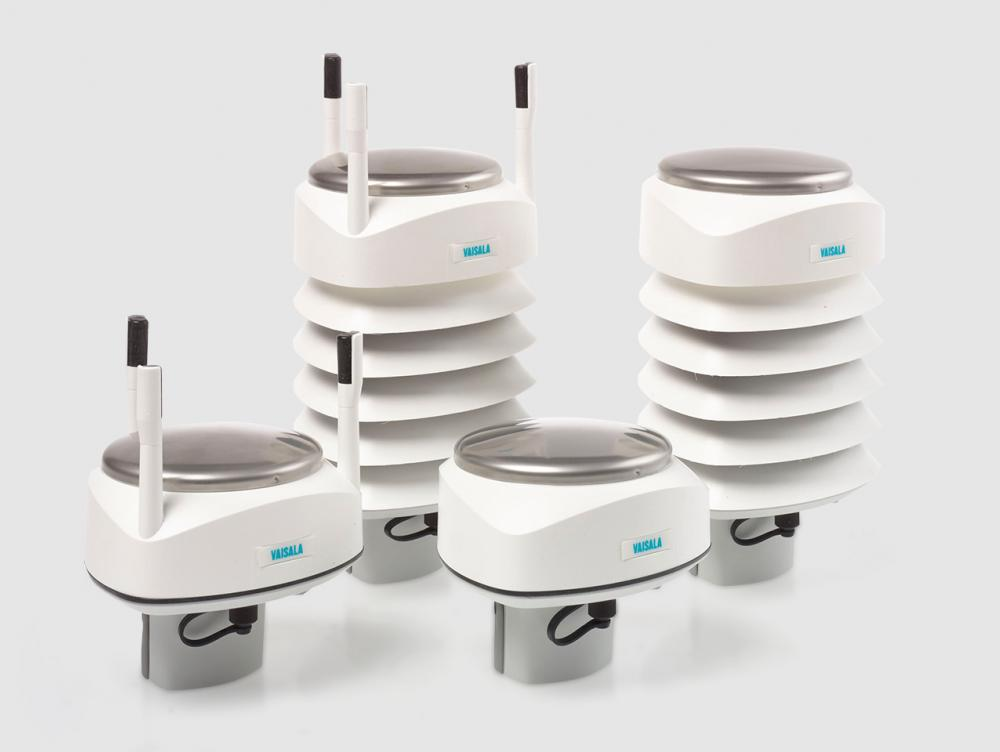
\includegraphics[scale=0.4]{meteo_station}
	\caption{Автоматическая метеостанция WXT530~\cite{wxt530}}
	\label{fig:lit_reiview:meteo:meteo_station}
\end{figure}

\subsection{Специальный принтер}
\label{sub:lit_review:spec_printer}
Специальный принтер предназначен для эксплуатации в составе мобильных вычислительных комплексов.
Может эксплуатироваться в процессе движения транспортных средств ~\cite{mp2200}.

Наиболее удобным для эксплуатации в машине КМУ является термопринтер. Термопринтеры гораздо более устойчивы к вибрациям и ударам, чем лазерные, матричные и струйные принтеры.

Корпус выполнен из металла, что обеспечивает стойкость к внешним механическим воздействиям.
Разъемы питания и интерфейсов (USB/LPT) принтера –высоконадежные «военные» байонетные металлические с металлической защитной заглушкой.
Интерфейс – высокоскоростной параллельный ECP/EPP и/или USB.

\begin{figure}[ht]
	\centering
	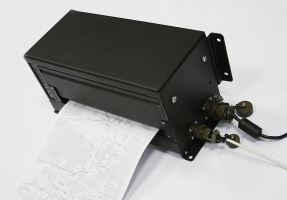
\includegraphics[scale=1.0]{printer}
	\caption{Специальный принтер~\cite{mp2200}}
	\label{fig:lit_reiview:spec_printer:printer}
\end{figure}


\section{Системное проектирование}
\label{sec:arch}

После тщательного изучения предметной области, постановки целей и выделения задач дипломного проектирования, была
разработана структурная схема системы функционального контроля ТС КМУ артиллерийского дивизиона.
Система разделена на несколько слабо связанных модулей.
Данная система представляет собой клиент серверную архитектуру~\cite{cl_s},
где АРМ является сервером и осуществляет проверку клиентов -- подключенных устройств.

\begin{figure}[ht]
	\centering
	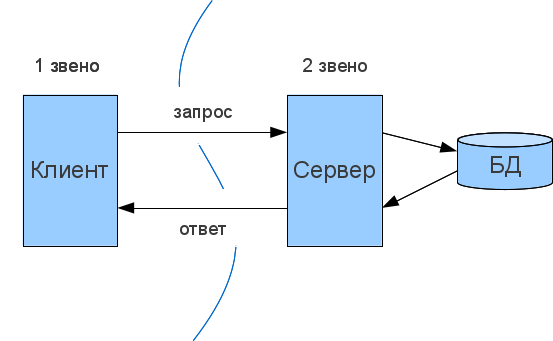
\includegraphics[scale=1.1]{client-s}
	\caption{Архитектура клиент-сервер~\cite{cl_s}}
	\label{fig:sec_arch:client}
\end{figure}

В системе имеются следующие блоки:
\begin{itemize}
	\item управляющий модуль
	\item блок тестирования и настройки ЛВС
	\item блок тестирования метеокомплекта
	\item блок тестирования навигационной системы
	\item блок автоматизации обнаружения устройств
	\item блок тестирования радиоканалов
	\item блок тестирования специального принтера
\end{itemize}

Данные модули являются довольно независимыми друг от друга. Из-за того, что системы тестирует множество различных
устройств, модули, работающие с периферийными устройствами имеют связь лишь с управляющим модулем.

Структурная схема, с изображением всех блоков и связей между ними, приведена на чертеже ГУИР.400201.065 С1.

Рассмотрим подробнее функциональные блоки системы.

\textit{Управляющий модуль} занимается обменом данными с остальными модулями, он занимается посылкой команд
тестирования, приемом и выводом информации от модулей, работающих с периферией. Также данный модуль отвечает за общение
с пользователем программы и обработкой поступающих от устройств диагностических данных.

Данный модуль общается с другими путем вызова публично доступных методов других модулей. Управляющий модуль может также
передавать данные и внешним модулям, посредством доступного и удобного API. Данный способ может быть полезен при
включении системы функционального контроля в более крупную, например, таковой системой является комплекс автоматизации
КМУ артиллерийского дивизиона.

Взаимодействие с пользователем осуществляется с помощью графического интерфейса, основанного на Qt виджетах. Передача
управления другим блокам осуществляется с помощью команд контекстного меню и кнопок графического интерфейса.

Управляющий блок позволяет:
\begin{itemize}
	\item взаимодействовать с блоком тестирования и настройки ЛВС
	\item взаимодействовать с блоком тестирования метеокомплекта
	\item получать доступ к функциям тестирования специального принтера
	\item осуществлять доступ к системе автообнаружения устройств
	\item получать доступ к модулю тестирования радиоканалов
	\item осуществлять тестирование системы навигации, путем взаимодействия с соответствующим модулем
	\item осуществлять логгирование событий и вывод статистики
	\item проводить контроль доступа к подсистемам функционального контроля
\end{itemize}

\textit{Блок управления пользовательским интерфейсом} отвечает за взаимодействие с пользователем с помощью средств Qt.
Блок управляет содержанием и поведением окон приложения.

\textit{Блок автоматизации обнаружения устройств} занимается обнаружением всех подключенных к системе устройств,
настройку параметров общения с ними, ведение списка подключенной периферии.

Данный блок имеет крайне важное значение в связи с тем, что до недавнего времени операторам АРМ приходилось настраивать
все подключенные устройства вручную.
Сложнее всего -- идентифицировать правильно подключенные к АРМ устройства, так как
зачастую они подключены через COM порты и имеют в системе практически идентичные названия(TTYS0, TTYS1 и т.д).

Данный блок имеет следующие составляющие:
\begin{itemize}
		\item библиотека доступных протоколов
		\item модуль сканирования подключенных устройств
		\item модуль идентификации подключенных устройств
		\item внешний интерфейс для добавления новых устройств в библиотеку. Предоставляет возможность расширения библиотеки протоколов.
		\item модуль настройки подключенных устройств
		\item модуль ведения отчетности о подключенных устройствах
\end{itemize}

Данный модуль обращается к библиотеке устройств(протоколов) и производит поиск данных устройств в системе.

При дальнейшем развитии проекта предполагает интерес вынесения функционала данного блока в область ядра ОС. К сожалению,
данный подход имеет сложности в виду необходимости предоставления исходных кодов вместе с продуктом, в связи с
требованиями лицензии GPL.

Блок автоматизации обнаружения устройств не производит тестирование и диагностику подключенных ТС. Данный модуль лишь
помогает установить требуемые параметры для общения согласно заданному протоколу(проверка четности, скорость передачи и
т.п.).

\textit{Блок тестирования специального принтера} осуществляет проверку работоспособности принтера экипажа. Данный модуль
позволяет проверить состояние принтера, проверить уровень чернил и настройку параметров печати путем оправки тестовой
страницы на печать.

\textit{Блок тестирования и настройки ЛВС} позволяет:
\begin{itemize}
	\item настроить ip адреса, используемые программой для общения к внешним устройствам, к другим машинам в
		ЛВС
	\item провести проверку работоспособности сети
	\item собирать различную диагностическую информацию о состоянии сети: процент потерянных
		пакетов, время отклика между узлами ЛВС
	\item вести статистику, используя полученные данные
	\item выводить полученные результаты на экран монитора, либо на печать
\end{itemize}

Все АРМ внутри КМУ подключены к ЛВС, также к сети подключены и такие устройства как радиостанции и некоторые датчики,
обменивающиеся информацией с АРМ с помощью протоколов стека TCP/IP.
Машина управления также может связаться с другими машинами комплекса, используя ЛВС.

\textit{Блок тестирования навигационной системы} позволяет провести функциональный контроль подключенных к АРМ устройств
навигации.

Комплексная навигационная система состоит из следующих устройств:
\begin{itemize}
	\item бесплатформенная навигационная система(БИНС)
	\item блок измерительный спутниковый (БИС)
	\item датчик пути цифровой(ДПЦ)
\end{itemize}

Напрямую система общается лишь с БИНС. Обмен информацией с БИС и ДПЦ идет через БИНС.
Данные устройства позволяют получать различную информацию о местоположении машины, получать информацию о наклоне
машины относительно плоскостей координат(крен, тангаж).

Информация с данных датчиков отображается на экран монитора, печатается на принтере либо сохраняется в файл для
дальнейшей обработки. Система имеет множество различных регистров, хранящих данные о скорости машины, пройденном пути и
т.п. Необходимо проверить доступность данной информации, верифицировать ее достоверность.

Данная система также может работать с системами GPS и GLONASS, поэтому также следует проверять следующие моменты:
\begin{itemize}
	\item доступность спутников
	\item величину сигнала со спутника
	\item автоматический поиск спутников
	\item верность полученной информации
	\item одновременное использование обеих систем навигации
	\item переключение на другую систему ввиду слабого или отсутствующего сигнала спутника
\end{itemize}

Используя имеющиеся датчики, КНС может получать данные о местоположении даже ввиду отсутствия GPS/GLONASS спутников в
зоне досягаемости.
Это достигается за счет использования одометров, гироскопов, акселерометров. Обработкой этих данных
занимается БИНС.
Поэтому необходимо также проверить правильность работы самого БИНС.

\textit{Блок тестирования радиоканалов} занимается тестированием и настройкой средств радиосвязи.

В машинах КМУ установлено несколько различных типов раций, общение с которыми имеет определенные отличия.
Рации имеют
различный тип внутреннего устройства, различный форм фактор, различный диапазон для передачи данных.

Общение через радиоканал может осуществляться как внутри машины, так и с другими машинами и объектами на местности.
Блок тестирования радиоканала позволяет проверить работу различных типов раций во всевозможных режимах работы.

Например, рация в КМУ может иметь следующие режимы работы:
\begin{itemize}
		\item общение точка-точка внутри машины
		\item режим конференц связи внутри машины
		\item режим общения с членом экипажа другой машины
\end{itemize}

В связи с данными сложностями, необходимо проверить следующие варианты работы системы:
\begin{itemize}
	\item работа в режиме точка-точка внутри машины
	\item возможность осуществления конференц связи
	\item проверка работы зашифрованного обмена
	\item обмен данными по радиоканалу
	\item возможность связи с другими машинами КМУ
	\item возможность обмена на всем спектре доступных частот
\end{itemize}

\textit{Блок тестирования метеокомплекта} позволяет проводить тестирование работы метеокомплекта, который имеется во
всех КМУ.

Метеокомплект предоставляет следующую информацию:
\begin{itemize}
	\item осадки
	\item атмосферное давление
	\item температура
	\item относительная влажность
	\item направление ветра
	\item скорость ветра
\end{itemize}

Необходимо проверить доступность всей вышеприведенной информации, проверить ее достоверность, провести настройку
устройства.



\section{Функциональное проектирование}
\label{sec:func}

\subsection{Класс \texttt{QTestPrinter}}
Класс \texttt{QTestPrinter} является реалиизацией блока тестирования специального принтера.
Данный класс выполняет поиск подлюченных принтеров, проверку правильности настроек принтера,
позволяет осуществить проверку состояния принтера путем печати тестовой страницы.

Класс \texttt{QTestPrinter} включает в себя следующие методы:

\begin{itemize}
	\item Метод \texttt{test} проводит процедуру тестирования принтера. Данный метод принимает ссылку на строку
		\texttt{sRez}. Данная строка служит для логгирования процесса тестирования устройства. Метод \texttt{test} производит
		проверку наличия принтера и корректности настроек его подкючения. В случае, если принтер подключен корректно, создается
		диалоговое окно для печати тестовой страницы. Для формирования тестовой страницы служит метод \texttt{print}, который
		связан с сигналом \texttt{paintRequested}. Сигнал \break\texttt{paintRequested} посылается при необходимости станартного
		класса Qt \texttt{QPrintPreviewDialog} сгенерировать изображения для предпросмотра\break печатаемых страниц.

	\item Метод \texttt{print} осуществляет формирование тестовой страницы и настройку параметров печати. \texttt{print}
		принимает в качестве параметра указатель на класс \texttt{QPrintPreviewDialog}, который используется для настройки
		параметров печати.
\end{itemize}

\subsection{Класс \texttt{VTest\_BINS3}}
Данный класс отвечает за тестирование БИНС, работающей по протоколу БИНС-3.

Класс \texttt{VTest\_BINS3} имеет следующие методы и внутренние переменные:
\begin{itemize}
	\item Переменная \texttt{m\_bReceiveMess81} является флагом, который выставляется при получении сообщения
		статуса БИНС-3. Сообщение статуса имеет идентификатор 0x81.

	\item Переменная \texttt{m\_bReceiveMess01} - флаг, отвечающий за получения сообщения с навигационными данными.
		Данное Сообщение имеет идентификатор 0x01.

	\item Метод \texttt{onReadFromBins} принимает полученную с БИНС дейтаграмму в виде \texttt{QByteArray}.
		и осуществляет определение типа полученной команды. После определения типа команды устанваливается
		соотетствующий флаг.

	\item Метод \texttt{onReadFromSocket} выполняет чтение данных из сокета, через который идет общение с БИНС,
		метод вызывается при появлении информации для чтения с БИНС(сигнал \texttt{readyRead}).
		Данный метод принимает полученную с БИНС дейтаграмму в виде \texttt{QByteArray}.
		При считывании байт команды дейтаграмма передается в метод \texttt{onReadFromBins} для определения типа
		команды.

	\item Метод \texttt{test} является основным методом класса \texttt{VTest\_BINS3}.\break Данный метод отвечает
		непосредственно за управление тестированием\break БИНС. Метод проверяет подключение БИНС, настройки и
		параметры подключения устройства. При успешном получении сообщения с навигационными данными и сообщения
		статуса, программа передает управление функциям \texttt{decodeMes01} и \texttt{decodeMes81} для
		получения более подробных данных о состоянии устройства.

	\item Метод \texttt{decodeMes01} отвечает за анализ сообщений с навигационными данными. Метод принимает
		дейтаграмму \texttt{sRez} в качестве входного параметра. Метод позволяет получить
		различные навигационные данные(угол крена, угол тангажа, модуль скорости и т.п.), получить информацию об
		источниках координат, получить информацию о единицах измерения величин и системе координат, проверить
		достоверность полученных данных.

	\item Метод \texttt{decodeMes81} позволяет получить подробную информацию о состоянии системы. Метод принимает
		ссылку на флаг исправности устройства \texttt{bIspr} и ссылку на дейтаграмму \texttt{sRez}. Полученную
		информацию можно разделить на следующие категории:
		\begin{itemize}
				\item информация о состоянии ДПЦ;
				\item информация о доступных спутниках и наличии навигационного решения;
				\item информация о состоянии и исправности БИС-3;
				\item информация о состоянии INS;
				\item информация о наличии неисправностей в работе гироскопа и блока акселлерометров.
		\end{itemize}

	\item Метод \texttt{getCurrentTime} служит для получения текущего времени.

	\item Сигнал \texttt{getAllMessFromBINS} извещает о том, что уже получено и сообщение статуса, и сообщение с
		навигационными данными.. Данный сигнал посылается из функции \texttt{onReadFromBins} при наличии
		одновременно установленных флагов
		\texttt{m\_bReceiveMess01} и \texttt{m\_ReceiveMess81}. Данный сигнал используется в методе
		\texttt{test} при асинхронном ожидании окончания чтения из БИНС.

	\item Переменные \texttt{m\_mes01} и \texttt{m\_mes81} являются переменными типов \texttt{\_KDG\_01} и
		\texttt{\_KDG\_81} соответственно. Данные типа представляют собой\break структуры, описанные в заголовочном
		файле \texttt{Protocol\_BINS3.h}. Переменные данных типов инкапсулируют в себе дейтаграммы
		соответствующего формата. Переменные \texttt{m\_mes01} и \texttt{m\_mes81} используются в функциях
		\texttt{decodeMes01} и \texttt{decodeMes81} соответственно для удобного доступа к различным полям в
		заголовках дейтаграмм.
\end{itemize}

\subsection{Класс \texttt{VTest\_KNS2}}
Данный класс отвечает за тестирование КНС, работающей по протоколу КНС-2.

Класс \texttt{VTest\_KNS2} имеет следующие методы и внутренние переменные:
\begin{itemize}
	\item Переменная \texttt{m\_sockReceive} используется для создания UDP сокета, связанного с КНС.

	\item Флаг \texttt{m\_bSignValidTime} используется при проверке достоверности навигационных данных.

	\item Переменная \texttt{m\_timeGPS} служит для хранения времени, полученного из КНС.

	\item Переменная \texttt{m\_bReceiveMess66} является флагом, который выставляется при получении статусного
		сообщения КНС-2. Статусное сообщение имеет идентификатор 0x66.

	\item Переменная \texttt{m\_bReceiveMess01} - флаг, отвечающий за получения сообщения с навигационными данными.
		Данное Сообщение имеет идентификатор 0x01.

	\item Метод \texttt{onReadFromKNS} принимает полученную с КНС дейтаграмму в виде \texttt{QByteArray}.
		и осуществляет определение типа полученной команды. После определения типа команды устанваливается
		соотетствующий флаг.

	\item Метод \texttt{onReadFromSocket} выполняет чтение данных из сокета, через который идет общение с КНС,
		метод вызывается при появлении информации для чтения с КНС(сигнал \texttt{readyRead}).
		Данный метод принимает полученную с МНСТО дейтаграмму в виде \texttt{QByteArray}.
		При считывании байт команды дейтаграмма передается в метод \texttt{onReadFromKNS} для определения типа
		команды.

	\item Метод \texttt{test} является основным методом класса \texttt{VTest\_KNS2}. Данный метод отвечает
		непосредственно за управление тестированием\break КНС. Метод проверяет подключение КНС, настройки и
		параметры подключения устройства. Устройство может быть подключено как через COM порт, так и через
		сокетное соединение. В зависимости от типа подключения устройства необходимо использовать
		соответствующую реализацию метода. Метод инициирует устнаовление соединения с устройством и в случае
		успеха начинает обмен данными с КНС. При успешном получении сообщения с навигационными данными и сообщения
		статуса, программа передает управление функциям \texttt{decodeMes01} и \texttt{decodeMes66} для
		получения более подробных данных о состоянии устройства. При корректности полученных навигационных
		данных устанавливается флаг \texttt{m\_bSignValidTime} и происходит запись времени в переменную класса
		\texttt{m\_timeGPS}.

	\item Метод \texttt{decodeMes01} отвечает за анализ сообщений с навигационными данными. Метод принимает
		дейтаграмму \texttt{sRez} в качестве входного параметра. Метод позволяет получить
		различные навигационные данные(угол крена, угол тангажа, модуль скорости и т.п.), получить информацию о
		cостоянии устройства, получить информацию о исправности различных датчиков КНС, проверить достоверность
		полученной от датчиков информации.

	\item Метод \texttt{decodeMes66} позволяет получить подробную информацию о состоянии системы. Метод принимает
		ссылку на флаг исправности устройства \texttt{bIspr} и ссылку на дейтаграмму \texttt{sRez}. Данная
		дейтаграмма может\break предоставлять следующую информацию:
		\begin{itemize}
				\item время до завершения операции;
				\item идентификатор текущей операции;
				\item флаги исправности датчиков и подсистем КНС.
		\end{itemize}

	\item Метод \texttt{testByMulticast} позволяет провести проверку наличия КНС в мультикаст группе в случае
		общения с устройством через ЛВС.

	\item Метод \texttt{getCurrentTime} служит для получения текущего времени.

	\item Сигнал \texttt{getAllMessFromKNS} извещает о том, что уже получено и сообщение статуса. Данный сигнал
		посылается из функции\break \texttt{onReadFromKNS} при наличии
		устновленного флага
		\texttt{m\_bReceiveMess01}. Данный сигнал используется в методах
		\texttt{test} и \texttt{testByMulticast} при асинхронном ожидании окончания чтения из КНС.

	\item Переменные \texttt{m\_mes01} и \texttt{m\_mes66} являются переменными типов \texttt{\_KDG\_01} и
		\texttt{\_KDG\_66} соответственно. Данные типа представляют собой\break структуры, описанные в заголовочном
		файле \texttt{Protocol\_KNS2.h}. Переменные данных типов инкапсулируют в себе дейтаграммы
		соответствующего формата. Переменные \texttt{m\_mes01} и \texttt{m\_mes66} используются в функциях
		\break
		\texttt{decodeMes01} и \texttt{decodeMes66} соответственно для удобного доступа к различным полям в
		заголовках дейтаграмм.
\end{itemize}

\subsection{Класс \texttt{VTest\_MNSTO}}
Данный класс отвечает за тестирование работы МНСТО. МНСТО работает по одноименному протоколу.

Класс \texttt{VTest\_MNSTO} имеет следующие методы и внутренние переменные:
\begin{itemize}
	\item Переменная \texttt{m\_sockReceive} используется для создания UDP сокета, связанного с МНСТО.

	\item Флаг \texttt{m\_bSignValidTime} используется при проверке достоверности навигационных данных.

	\item Переменная \texttt{m\_timeGPS} служит для хранения времени, полученного из МНСТО.

	\item Переменная \texttt{m\_bReceiveMess02} является флагом, который выставляется при получении сообщения с
		навигационными данными. Данное сообщение имеет идентификатор 0x02.

	\item Переменная \texttt{m\_bReceiveMess01} - флаг, отвечающий за получения сообщения с данными о состоянии
		устройства.
		Данное Сообщение имеет идентификатор 0x01.

	\item Метод \texttt{onReadFromKNS} принимает полученную с МНСТО дейтаграмму в виде \texttt{QByteArray}.
		и осуществляет определение типа полученной команды. После определения типа команды устанваливается
		соотетствующий флаг.

	\item Метод \texttt{onReadFromSocket} выполняет чтение данных из сокета, через который идет общение с МНСТО,
		метод вызывается при появлении информации для чтения с МНСТО(сигнал \texttt{readyRead}).
		Данный метод принимает полученную с МНСТО дейтаграмму в виде \texttt{QByteArray}.
		При считывании байт команды дейтаграмма передается в метод\break \texttt{onReadFromMNSTO} для определения типа
		команды.

	\item Метод \texttt{test} является основным методом класса \texttt{VTest\_MNSTO}. Данный метод отвечает
		непосредственно за управление тестированием\break КНС. Метод проверяет подключение МНСТО, настройки и
		параметры подключения устройства. Устройство может быть подключено как через COM порт, так и через
		сокетное соединение. В зависимости от типа подключения устройства необходимо использовать
		соответствующую реализацию метода. Метод инициирует устнаовление соединения с устройством и в случае
		успеха начинает обмен данными с МНСТО. При успешном получении сообщения с навигационными данными и сообщения
		статуса, программа передает управление функциям \texttt{decodeMes02} и \texttt{decodeMes01} для
		получения более подробных данных о состоянии устройства. При корректности полученных навигационных
		данных устанавливается флаг \texttt{m\_bSignValidTime} и происходит запись времени в переменную класса
		\texttt{m\_timeGPS}.

	\item Метод \texttt{decodeMes02} отвечает за анализ сообщений с навигационными данными. Метод принимает
		дейтаграмму \texttt{sRez} в качестве входного параметра. Метод позволяет получить
		различные навигационные данные(угол крена, длина пройденного пути, скорость и т.п.),
		проверить достоверность полученной от датчиков информации.

	\item Метод \texttt{decodeMes01} позволяет получить подробную информацию о состоянии системы. Метод принимает
		ссылку на дейтаграмму \texttt{sRez}. Данная
		дейтаграмма может предоставлять следующую информацию:
		\begin{itemize}
				\item состояние МНСТО;
				\item состояние БИН;
				\item сотояние БИС;
				\item состояние ДПЦ.
		\end{itemize}

	\item Метод \texttt{testByMulticast} позволяет провести проверку наличия МНСТО в мультикаст группе в случае
		общения с устройством через ЛВС.

	\item Метод \texttt{getCurrentTime} служит для получения текущего времени.

	\item Сигнал \texttt{getAllMessFromMNSTO} извещает о том, что уже получено и сообщение статуса. Данный сигнал
		посылается из функции\break \texttt{onReadFromMNSTO} при наличии
		устновленного флага\break
		\texttt{m\_bReceiveMess02}. Данный сигнал используется в методах
		\texttt{test} и\break \texttt{testByMulticast} при асинхронном ожидании окончания чтения из МНСТО.

	\item Переменные \texttt{m\_mes01} и \texttt{m\_mes02} являются переменными типов \texttt{\_KDG\_01} и
		\texttt{\_KDG\_02} соответственно. Данные типа представляют собой структуры, описанные в заголовочном
		файле \texttt{Protocol\_MNSTO.h}. Переменные данных типов инкапсулируют в себе дейтаграммы
		соответствующего формата. Переменные \texttt{m\_mes01} и \texttt{m\_mes02} используются в функциях
		\texttt{decodeMes01} и \texttt{decodeMes02} соответственно для удобного доступа к различным полям в
		заголовках дейтаграмм.
\end{itemize}

\subsection{Блок журналирования}
Данный блок осуществляет ведение журнала функционального тестирования устройств. Блок состоит из следующих компонентов:

\subsubsection{Структура \texttt{DeviceInfo}}
Структура \texttt{DeviceInfo} представляет собой запись о результатах тестирования одного устройства.
Данная структура содержит следующие поля:
\begin{itemize}
	\item \texttt{deviceName} -- поле, в котором хранится имя тестируемого устройства;
	\item \texttt{resultMessage} -- поле, в котором хранится информация о результатах тестирования;
	\item \texttt{additionalInfo} -- поле, предназначенное для хранения дополнительной информации о
		результатах тестирования устройства;
	\item \texttt{hasError} -- флаг, который указывает на наличие ошибок, обнаруженных в ходе
		тестирования устройства.
\end{itemize}

\subsubsection{Класс \texttt{JournalEntry}}
Данный класс используется для формирования записи о результатах тестирования устройств.

Данный класс содержит следующие методы и переменные класса, в нем также объявлены следующие структуры:
\begin{itemize}
	\item Переменная \texttt{date} служит для хранения информации о времени проведения тестирования.

	\item Переменная \texttt{devices} является списком, хранящим структуры\break \texttt{DeviceInfo}. Таким образом,
		данный список хранит информацию о результатах последнего тестирования устройств.

	\item Метод \texttt{addDevice} осуществляет добавление нового устройства к списку \texttt{devices}. Данный метод
		принимает в качестве параметров структуру типа \texttt{DeviceInfo}.

	\item Метод \texttt{getDate} служит для получения значения переменной \texttt{date}.

	\item Метод \texttt{getDevices} возвращает список устройст \texttt{devices}.
\end{itemize}

\subsubsection{Класс \texttt{Journal}}
Класс \texttt{Journal} служит для записи результатов тестирования в журнал. Для удобства операций с жураналом
тестирования, результаты тестирования хранятся в формате JSON. Класс \texttt{Journal} содержит следующие методы:
\begin{itemize}
	\item Метод \texttt{store} служит для добавления новой записи в журнал тестирования. Перед добавлением новой
		записи \texttt{JournalEntry} в файл, она конвертируется в JSON строку c помощью метода \texttt{asJSON}.
		Перед записью в файл, происходит считывание всего файла, после чего новая запись добавляется к массиву
		записей с помощью метода \texttt{appendEntryToArray}.

	\item Метод \texttt{asJSON} принимает запись типа \texttt{JournalEntry} и преобразует ее в JSON строку.
		Все данные структуры, включая имена полей, преобразуются в удобный для чтения текст. Также в
		результирующую строку добавляется информация о дате проведения тестирования.

	\item Метод \texttt{appendEntryToArray} принимаетс сылки на журнал тестирования \texttt{jsonArray} и новую
		запись \texttt{jsonJournalEntry}. Данный метод осуществляет добавление новой записи в массив
		\texttt{jsonArray}.
\end{itemize}

\subsection{Класс \texttt{OffLineFuncControl}}
Данный класс представляет собой управляющий модуль.\break \texttt{OffLineFuncControl}осуществляет взаимодействие с элементами графического
интерфейса, а также с классами, отвечающими за тестирование периферийных устройств.
Данный класс включает в себя следующие методы и переменные:
\begin{itemize}
	\item Переменная \texttt{m\_pTreeDevice}
	\item Переменная \texttt{m\_pBtStart}
	\item Переменная \texttt{m\_pBtPrint}
	\item Переменная \texttt{m\_pBtSettings}
	\item Переменная \texttt{m\_pBtJournal}
	\item Переменная \texttt{m\_pBtTestKS}
	\item Переменная \texttt{m\_pBtExit}

	\item Переменная \texttt{m\_bStartTest}
	\item Переменная \texttt{m\_Menu}
	\item Переменная \texttt{m\_pActInfo}

	\item Переменная \texttt{m\_syncroTime}

	\item Переменная \texttt{m\_sockReceiveUpdate}

	\item Переменная \texttt{m\_sockReceiveUpdate}

	\item Переменная \texttt{m\_pActSetParam}
	\item Переменная \texttt{m\_pMenuSNS}
	\item Переменная \texttt{m\_pActSNS\_GPS\_GLONASS}
	\item Переменная \texttt{m\_pActSNS\_GPS}
	\item Переменная \texttt{m\_pActSNS\_GLONASS}

	\item Переменная \texttt{m\_pActSetTimeOnServer}
	\item Переменная \texttt{m\_pActSetTimeFromGPS}

	\item Переменная \texttt{ntpHelperPtr}

	\item Переменная \texttt{timePickWidget}
	\item Переменная \texttt{dateTimeEdit}
	\item Переменная \texttt{m\_pBtConfirmDate}

	\item Метод \texttt{messageReceived} служит для анализа полученных команд и выполнения соответствующих действий
		в ответ на них.

	\item Метод \texttt{resizeEvent} вызывается при изменении размеров окна. Данный метод служит для оптимального
		изменения положения элементов окна в соответствии с текущим размером окна.

	\item Метод \texttt{closeEvent} служит для переопределения стандартного метода закрытия окна. Данный метод
		служит для отправки служебных сообщений имитаторам устройств перед завершением программы.

	\item Метод \texttt{loadDevices} используется для добавления устройств в список подключенных устройств.

	\item Метод \texttt{receiveSignalUpdate} срабатывает после получения сигнала \texttt{readyRead} от
		\texttt{m\_sockReceiveUpdate}. Данный метод служит для получения дейтаграмм. После получения каждой
		дейтаграммы управление передается методу \texttt{loadDevices} для дальнейшей обработки.

	\item Метод \texttt{onTestARM} проверяет корректность номера текущего АРМ и передает управление методу
		\texttt{test} класса \texttt{QTestARM} для проведения тестирования АРМ.

	\item Метод \texttt{onChangeCheckDevice} используется при изменении состояния чекбокса, отвечающего за включение
		устройства в список для тестирования.

	\item Метод \texttt{onStart} вызывается при нажатии кнопки \texttt{m\_pBtStart}. Данный метод служит для начала
		процесса функционального тестирования выбранных устройств.

	\item Метод \texttt{onMenu} срабатывает при вызове меню. Данный метод служит для вывода определенных пунктов
		меню, которые зависят от типа конкретного устройства.

	\item Метод \texttt{onInfo} срабатывает при выводе информационного сообщения. Данный метод вызывается при
		срабатывании триггера \texttt{m\_pActInfo}. Метод получает id текущего устройства и передает выполнение
		методу \texttt{onInfoDevice}.

	\item Метод \texttt{onInfoDevice} связан с кнопкой \texttt{pBtInfo}. Данный метод служит для предоставления
		информации о выбранном устройстве.

	\item Метод \texttt{onPrint}
	\item Метод \texttt{onJournal} служит для вызо%------
	\item Метод \texttt{print}
	\item Метод \texttt{onSettings}
	\item Метод \texttt{onTestKS}
	\item Метод \texttt{onManualSetTime} вызывается при срабатывании триггера \texttt{m\_pActSetTimeOnServer}.
		Данный метод выводит на экран\break \texttt{timePickWidget}.

	\item Метод \texttt{onGetTimeFromGps} вызывается при срабатывании триггера \texttt{m\_pActGetTimeFromGps}.
		Данный метод позволяет получить время, используя данные, полученные с помощью GPS. Полученные данные
		хранятся в переменной \texttt{dateTimeEdit}.

	\item Метод \texttt{onSelectTime} устанавливает время на сервере с помощью метода \texttt{setServerTime}. Метод
		\texttt{onSelectTime} вызывается при нажатии кнопки {m\_btConfirmDate}.
		метод \texttt{setServerTime} передается время полученное в результате вызова внутреннего метода
		\texttt{dateTime} объекта \texttt{dateTimeEdit}.

	\item Метод \texttt{saveRezTest} служит для сохранения результатов тестирования устройств.
	\item Метод \texttt{initNtp} инициалирует \texttt{ntpHelperPtr}. Данный метод позволяет установить соединение с
		ntp сервером.

	\item Метод \texttt{setServerTime} позволяет установить время на ntp сервере. Для этого используются методы
		объекта \texttt{ntpHelperPtr}.

	\item Метод \texttt{onTestTimeServer}
\end{itemize}


\section{ПРОГРАММА И МЕТОДИКА ИСПЫТАНИЙ}
\label{sec:test}
Тестирование разрабатываемых программных продуктов является\break крайне важным процессом. Тестирование позволяет избежать
лишних затрат на разработку, так как ошибки, возникающие в процессе разработки ПО,\break вскрываются как можно раньше. Также
исправление как можно большего количества ошибок перед релизом позволяет избежать затрат на исправление ошибок после
внедрения ПО.

Тестирование позволяет не только выявить ошибки в программном коде, но и вычислить фрагменты кода, требующие
оптимизации. Выполнение этой функции облегчают инструменты трассировки и профилирования кода.

Тестирование программы проводилось на компьютере со следующими характеристиками:
\begin{itemize}
	\item центральный процессор -- Intel Core i5-5200U с тактовой частотой 2.20ГГц;
	\item объем оперативной памяти -- 4 ГБ;
	\item операционные системы: ArchLinux x86\_64, Windows 10 x86\_64\break Education Edition.
\end{itemize}

\subsection{Отладчик GDB}
\label{sec:test:gdb_debug}
В качестве отладчика был выбран GDB, так как он может быть использован для тестирования как и в ОС Linux, так и в ОС
Windows. GDB также позволяет использовать отладчик, используя графический интерфейс. Для этого можно использовать
подключение GDB в качестве инструмента отладки к многим популярным IDE.

Для запуска отладчика необходимо наличие в отлаживаемой программе таблицы символов. Для этого требуется компиляция
проекта в debug режиме. В release версии таблица символов удаляется для экономии места и затруднения эксплуатации
возможных уязвимостей.
\begin{figure}[htb]
	\centering
	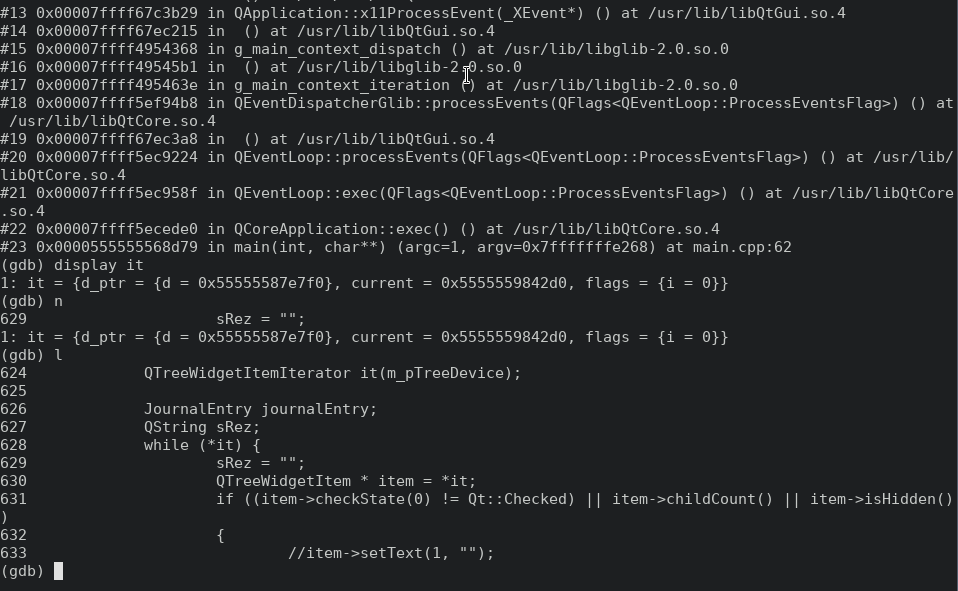
\includegraphics[scale=0.6]{gdb}
	\caption{Работа с gdb через консоль}
	\label{fig:test:gdb_debug:gdb}
\end{figure}

В процессе отладки большинство ошибок было устранено при использовании gdb через консоль. Пример окна отладки
представлен на рис. \ref{fig:test:gdb_debug:gdb}. При отладке пригодились следующие возможности gdb:
\begin{itemize}
	\item просмотр кода отлаживаемой функции;
	\item механизм контрольных точек;
	\item просмотр состояния переменных во время исполнения;
	\item постоянное отображения выбранных переменных с помощью команды \texttt{display};
	\item вывод стека вызова функций;
	\item изменение содержимого переменных в ходе отладки;
	\item анализ причины внезапного закрытия приложения с помощью анализа core файлов.
\end{itemize}

С помощью gdb удалось выявить ряд ошибок, которые были связаны с доступом за пределы выделенной памяти, использованием
данных через указатель после освобождения памяти, формированием неправильных выходных данных алгоритмами.

\subsection{Использование Valgrind для отладки использования памяти}
\label{sec:test:valgrind}
В ходе разработки и отладки дипломного проекта были выявлены проблемы связанные с утечкой памяти, повторным
использованием памяти, использованием неинициализированнной памяти, использованием памяти, которая находится за
пределами выделенного блока. Для решения этих и других проблем, после анализа существующих инструментов отладки и
профилирования, было принято решение использовать пакет Valgrind, который распространяется под лицензией GPL.

Valgrind представляет собой виртуальную машину, на которой происходит исполнение программы и ее анализ с помощью
различных инструментов, входящих в пакет Valgrind. Данная виртуальная машина использует метод динамической
перекомпиляции для запуска программы. Valgrind транслирует программу в промежуточное представление, после преобразования
для отладки программы могу быть использованы инструменты, входящие в Valgrind, данные инструменты проводят необходимые
преобразования программы, находящейся в промежуточном представлении, после чего происходит трансляция программы в
машинный код.

Преобразования значительно замедляет работу программы. Разработанная программа не содержит алгоритмов, требующих больших
затрат ресурсов вычислительной системы, поэтому использование инструментов, входящих в пакет Valgrind, является
целесообразным.

Пакет Valgrind содержит в себе набор инструментов для отладки и профилирования программы. В ходе разработки и отладки
проекта были использован инструмент Memcheck. Далее будет приведен краткий обзор этого инструмента.
\begin{figure}[htb]
	\centering
	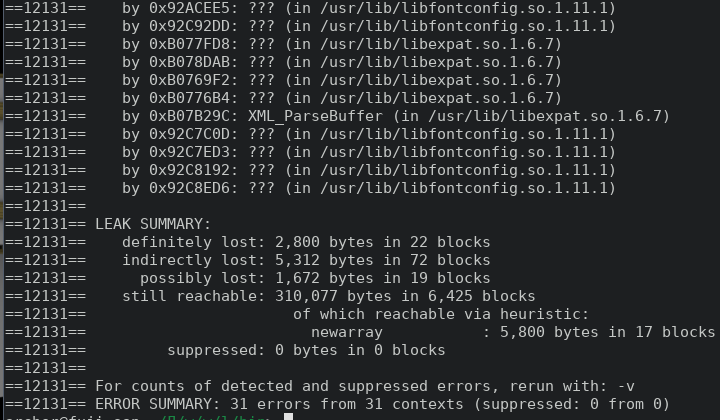
\includegraphics[scale=0.8]{memcheck}
	\caption{Результаты анализа программы с помощью Memcheck}
	\label{fig:test:valgrind:memcheck}
\end{figure}

Инструмент Memcheck (рис. \ref{fig:test:valgrind:memcheck}) используется для анализа ошибок, связанных с некорректной работой с памятью. Данный инструмент
используется по умолчанию в пакете Valgrind. Memcheck вставляет дополнительный код вокруг инструкций, которые
производят выделение памяти, также производит маркировку памяти. Memcheck помечает участки памяти, находящиеся за
границами выделенных блоков как некорректные, что позволяет детектировать ошибки, связанные с выходом за пределы
выделенной области памяти. Memcheck помечает блоки памяти флагами валидности (определяет, была ли память
проинициализированна) и адресуемости (определяет, относится ли данный участок памяти к выделенному блоку). Изменение состояния маркеров в ходе выполнения программы и
анализ данных маркеров позволяют выполнять обнаружение следующих ошибок при работе с памятью:
\begin{itemize}
	\item утечка памяти;
	\item доступ к памяти за пределами выделенного блока;
	\item доступ к памяти после ее освобождения;
	\item использование неинициализированнной памяти.
\end{itemize}

\subsection{Использование программ-имитаторов}
Работа разработанной системы функционального контроля\break технических средству КМУ артиллерийского дивизиона тесно связана с
взаимодействием с различным оборудованием. Многие из технических средств имеют большие габариты, требуют подключения
через интерфейс RS-232 либо получение данных от них требует значительных временных затрат. Тестировать работу программы
с реальным оборудованием в \company~возможно либо в специальном помещении, выполняющем роль тестового полигона, либо
непосредственно на боевой машине. Рассмотрим недостатки и преимущества каждого из данных подходов.

Тестовый полигон представляет собой помещение с десятью компьютерами, к каждому из которых подключена различная
периферия, используемая в армейских подразделениях. Данный кабинет удобно использовать в первую очередь проектным командам для
совместного тестирования работы программ на реальном оборудовании, обсуждения проблем, возникающих при работе с
оборудованием, и рассмотрения новых путей их решения. Недостатком работы на тестовом полигоне является сложность
подключения большого количества устройств к компьютеру для проведения тестирования работы системы. Другими недостатками
являются: невозможность постоянной работы на полигоне, ввиду использования полигона несколькими командами, сложность
коммуникации с коллегами, ввиду нахождения полигона вдалеке от помещений разработчиков.

Тестирование работы программы на боевой машине позволяет проверить работу программы непосредственно в месте, где она
будет впоследствии развернута. Данный подход актуален на финальных стадиях разработки системы, когда необходимо
проверить нюансы работы в среде, близкой к условиям эксплуатации. В процессе тестирования в данной системе возможно
обнаружить сложнодетектеруемые в других условиях ошибки, такие как проблемы взаимодействия компьютеров в локальной сети
машины, либо проблемы в работе некоторых устройств тестовой среды. Данная среда не предназначена для разработки
программ, так как в машинах отсутствует связь с сетью Интернет, техника доступна лишь на небольшое количество времени и
может находиться вдали от офиса разработки.

Для повышения производительности труда и абстрагирования от работы реальных физических устройств в компании \company~были
разработаны специальные программы-имитаторы. Данные программы позволяют создавать виртуальные устройства, работающие по
необходимо протоколу. Подключение программ-имитаторов к системе осуществляется либо через виртуальные последовательные
порты, либо через сокетное соединение. Программы-имитаторы принимают сообщения от разрабатываемых программных модулей и
автоматически формируют соответствующие ответные сообщения. Также разработчик может настроить параметры устройства и
сформировать желаемую команду через графический интерфейс программы-имитатора (рис.\ref{fig:test:imitators:imitator}).
\begin{figure}[htb]
	\centering
	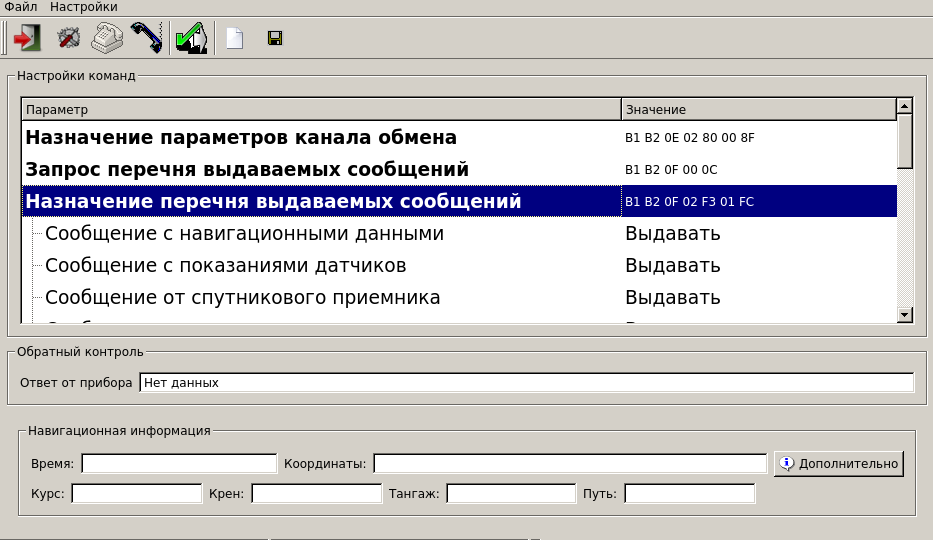
\includegraphics[scale=0.65]{imitator}
	\caption{Имитатор устройства, использующего протокол БИНС-3}
	\label{fig:test:imitators:imitator}
\end{figure}


\section{Руководство пользователя}
\label{sec:guide}

Данное программное обеспечение призвано для упрощения процесса проведения функционального ТС КМУ артиллерийского
дивизиона.\break
Программное обеспечение используется в составе комплекса программ для автоматизации АРМ.
Комплекс программ устанавливается на все АРМ КМУ артиллерийского дивизиона.

В данном разделе приведено руководство оператора АРМ по использованию системы функционального контроля.
Руководство включает в себя требования к аппаратному и программному обеспечению, последовательность запуска, выполнения
и завершение программы функционального контроля, а также приведены сообщения, возникающие при функционировании программы
с указанием возможных команд по управлению процессом выполнения программы.

\subsection{Требования к аппаратному и программному обеспечению}
\label{sub:guide:reqs}

Так как разработанное ПО используется в составе комплекса программ для автоматизации АРМ, ниже приведены требования к
аппаратному и программному обеспечению для работы всего программного комплекса.

Программный комплекс устанавливается на ПЭВМ и бортовую ЭВМ.

ПЭВМ должна иметь следующие характеристики:
\begin{itemize}
	\item центральный процессор -- Intel Pentium с частотой не менее 1,90 ГГц;
	\item объем оперативной памяти -- 4 ГБ;
	\item объем накопителя на жестком диске, SSD -- не менее 256 ГБ;
	\item сетевой адаптер -- Ethernet 10/100/1000 Мбит/с;
	\item порт USB 2.0 -- 2 шт.;
	\item порт RS232/422/485 -- 4 шт.;
	\item порт DVI -- 1 шт.
\end{itemize}

Бортовая ЭВМ должна иметь следующие характеристики:
\begin{itemize}
	\item центральный процессор -- Intel с частотой не менее 1.6 ГГц;
	\item объем оперативной памяти -- не менее 4 ГБ;
	\item сенсорный экран -- размер не менее 10 дюймов (разрешение не менее 1280х800);
	\item объем накопителя на жестком диске, SSD -- не менее 240 ГБ;
	\item сетевой адаптер -- Ethernet 10/100/1000 Мбит/с не менее 2 шт.;
	\item порт USB 2.0 -- не менее 2 шт.;
	\item порт RS232 -- не менее 1 шт.
\end{itemize}

Для загрузки ПО требуется внешний привод DVD-ROM с возможностью подключения к порту USB.
В меню настроек BIOS компьютеров первым устройством должно быть установлено устройство чтения DVD -- ROM.
Программа функционального контроля функционирует в сети\break Ethernet с пропускной способностью 10/100/1000 Мбит/с.
Дополнительно для функционирования ПЭВМ должно быть установлено следующее периферийное оборудование:

\begin{itemize}
	\item принтер промышленный;
	\item видеомонитор;
	\item клавиатура;
	\item манипулятор графической информации.
\end{itemize}

Для функционирования программы функционального контроля должна быть установлена 64-разрядная
операционная система Windows 7\break Professional или Windows 7 Ultra.

\subsection{Установка программного обеспечения}
\label{sub:guide:intstallation}

Данное ПО предназначено для использования в составе программного комплекса по автоматизации АРМ КМУ
артиллерийского дивизиона.
Установка программного комплекса на ЭВМ КМУ артиллерийского дивизиона в данном разделе
рассмотрена не будет.

Для использования в тестовых и демонстрационных целях система\break функционального контроля может быть установлена и
использоваться отдельно от остального комплекса.
В этом случае для установки достаточно скопировать содержимое диска
с ПО на компьютер.

\subsection{Руководство по использованию системы}
\label{sub:guide:user_guide}

При использовании системы в составе программного комплекса, запуск программы осуществляется с помощью соответствующих
элементов графического интерфейса главного окна управляющей программы комплекса.

Запуск программы тестирования устройств
осуществляется запуском\break файла OfflinefunctionControl.exe, который находится в
подкаталоге bin каталога системы функционального контроля.
В результате запуска программы отобразится главное окно <<Функциональный контроль>> программы, приведенное на рис.
\ref{fig:guide:user_guide:main_window}.
\begin{figure}
	\centering
	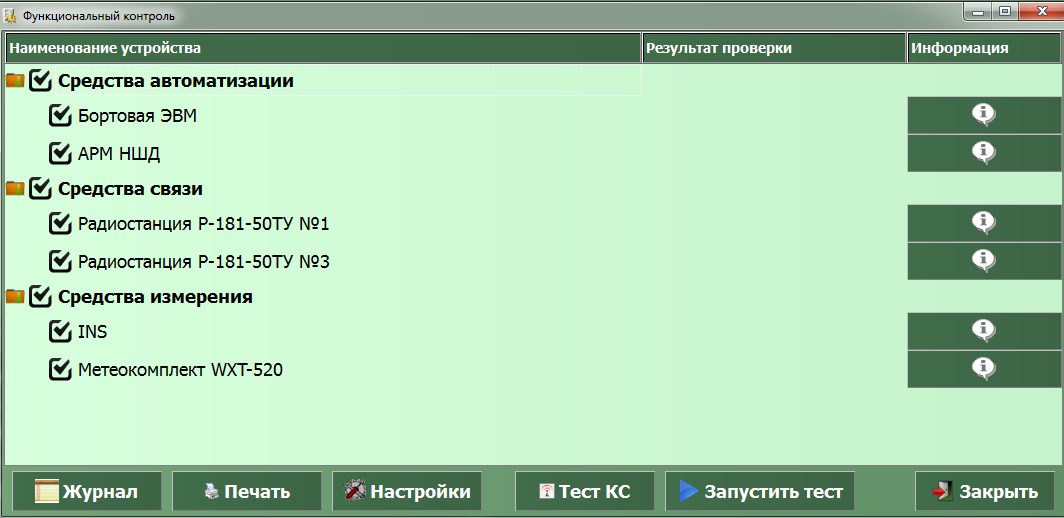
\includegraphics[scale=0.35]{main_window}
	\caption{Окно <<Функциональный контроль>>}
	\label{fig:guide:user_guide:main_window}
\end{figure}

Окно <<Функциональный контроль>> содержит список тестируемых технических средств
(наименование и количество устройств могут изменяться в зависимости от настроек АРМ).
Слева от наименования устройства имеется поле для установки флажка.
При нажатии кнопки <<Запустить тест>> запускаются тесты, отмеченные флажками.
При установке (снятии) флажка <<Средства автоматизации>>, <<Средства связи>>,
<<Средства измерения>> автоматически
устанавливаются (снимаются) флажки всех устройств, входящих в эту группу.
Тесты могут запускаться как по одному, так и все одновременно.
Результаты тестирования отображаются в столбце <<Результат проверки>> в виде сообщений:
\begin{itemize}
		\item <<Исправно>> (зеленого цвета);
		\item <<Неисправно>> (красного цвета);
		\item <<Порт занят>> (красного цвета).
\end{itemize}

При нажатии кнопки в столбце <<Информация>> открывается окно с подробной информацией о результатах проверки,
например, <<Бортовая ЭВМ>> (рис. \ref{fig:guide:user_guide:on_info}).
\begin{figure}[ht]
	\centering
	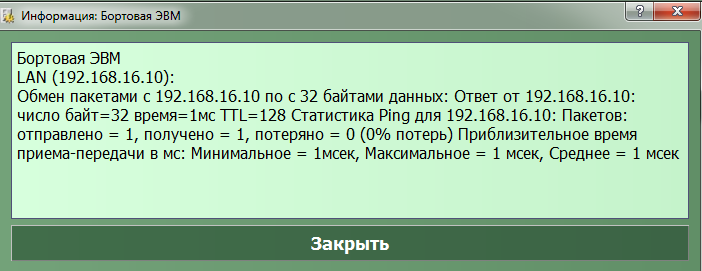
\includegraphics[scale=0.40]{on_info}
	\caption{Окно <<Информация: Бортовая ЭВМ>>}
	\label{fig:guide:user_guide:on_info}
\end{figure}
Для выхода из окна <<Информация: Бортовая ЭВМ>> нажать кнопку <<Закрыть>>.

Для тестирования каналов обмена данными необходимо нажать кнопку <<Тест КС>> (см. рис.
\ref{fig:guide:user_guide:main_window}).
В результате выполнения команды отобразится окно <<Тест каналов связи по радиостанциям Р–180/181>>, приведенное на рис.
\ref{fig:guide:user_guide:on_test_cs}.
\begin{figure}[ht]
	\centering
	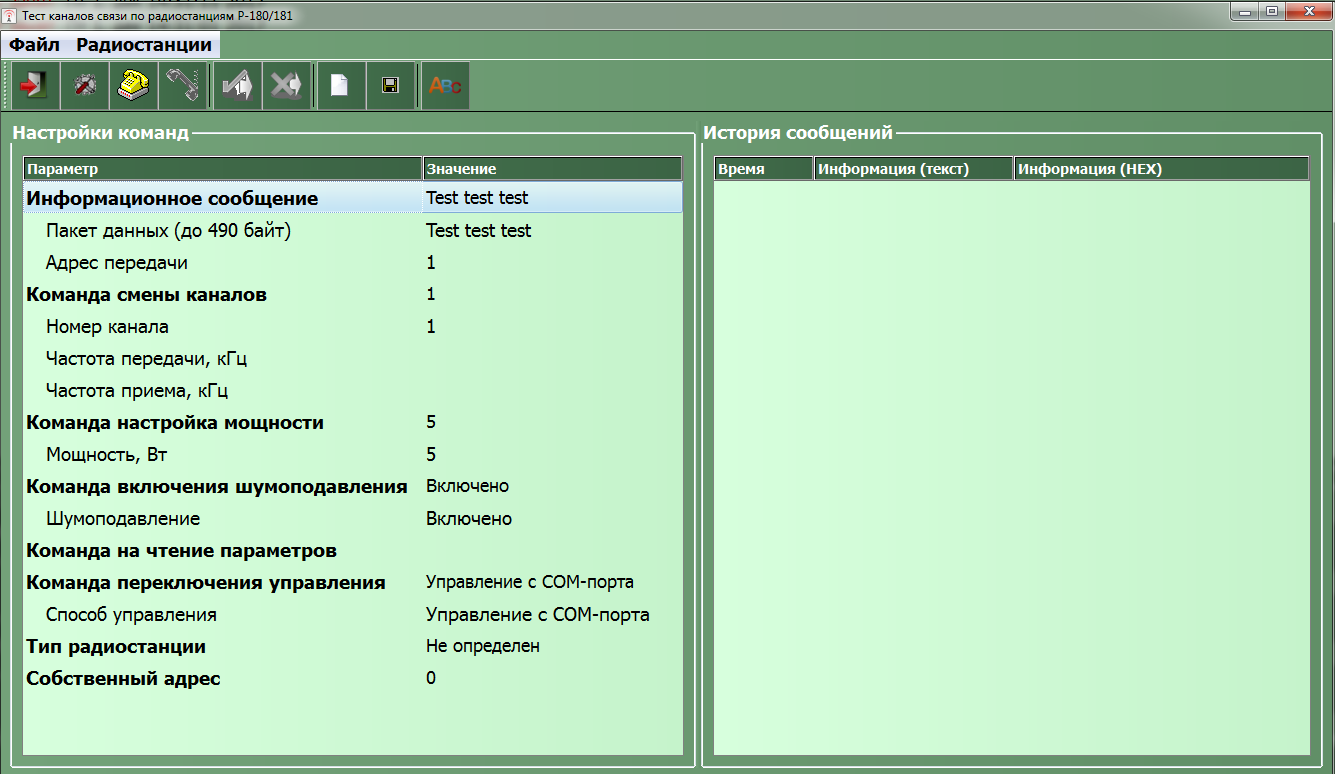
\includegraphics[scale=0.32]{on_test_cs}
	\caption{Окно <<Тест каналов связи по радиостанциям Р–180/181>>}
	\label{fig:guide:user_guide:on_test_cs}
\end{figure}
В левой части окна (см. рис. \ref{fig:guide:user_guide:on_test_cs}) отображается таблица <<Настройки команд>> с параметрами и значениями команд.
В правой части окна отображается таблица <<История сообщений>>, в которой хранится время получения сообщения.
В верхней части окна находится панель инструментов с кнопками, предназначенными для вызова требуемых функций.

Cлева направо на панели инструментов (см. рис. \ref{fig:guide:user_guide:on_test_cs}) расположены\break кнопки: <<Выход>>,
<<Настройки>>, <<Открыть порт>>, <<Закрыть порт>>,
<<Отправить сообщение>>, <<Очистить историю сообщений>>,
<<Сохранить историю сообщений>>, <<Режим ввода>>.

В меню <<Файл>> могут выполняться следующие команды:
\begin{itemize}
	\item <<Настройки>>;
	\item <<Открыть порт>>;
	\item <<Закрыть порт>>;
	\item <<Показать историю сообщений>>;
	\item <<Сохранить историю сообщений>>;
	\item <<Выход>>.
\end{itemize}

Для настройки порта нажать кнопку <<Настройки>> на панели инструментов (см. рис. \ref{fig:guide:user_guide:on_test_cs}) или выполнить команду
<<Настройки>> из меню <<Файл>>.
В результате выполнения команды отобразится окно, приведенное на рис. \ref{fig:guide:user_guide:port_config}.
\begin{figure}[htb]
	\centering
	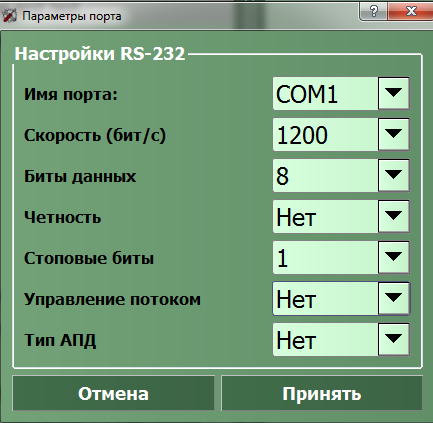
\includegraphics[scale=0.35]{port_config}
	\caption{Настройка параметров порта}
	\label{fig:guide:user_guide:port_config}
\end{figure}
Для проверки канала связи необходимо выдать информационное сообщение, для чего нажать кнопку <<Отправить сообщение>> на
панели инструментов окна <<Тест каналов связи по радиостанциям Р–180/181>> (см. рис.
\ref{fig:guide:user_guide:on_test_cs}) или выполнить команду <<Отправить сообщение>> из контекстного меню.
Переданное сообщение отображается в таблице <<История сообщений>>, в которой отображаются и полученные сообщения от абонента.

По нажатию кнопки <<Печать>> в окне <<Функциональный контроль>>
(см. рис. \ref{fig:guide:user_guide:main_window}) формируется для просмотра и выдачи на принтер отчет
о проведенном функциональном контроле (рис. \ref{fig:guide:user_guide:on_print}).
\begin{figure}[htb]
	\centering
	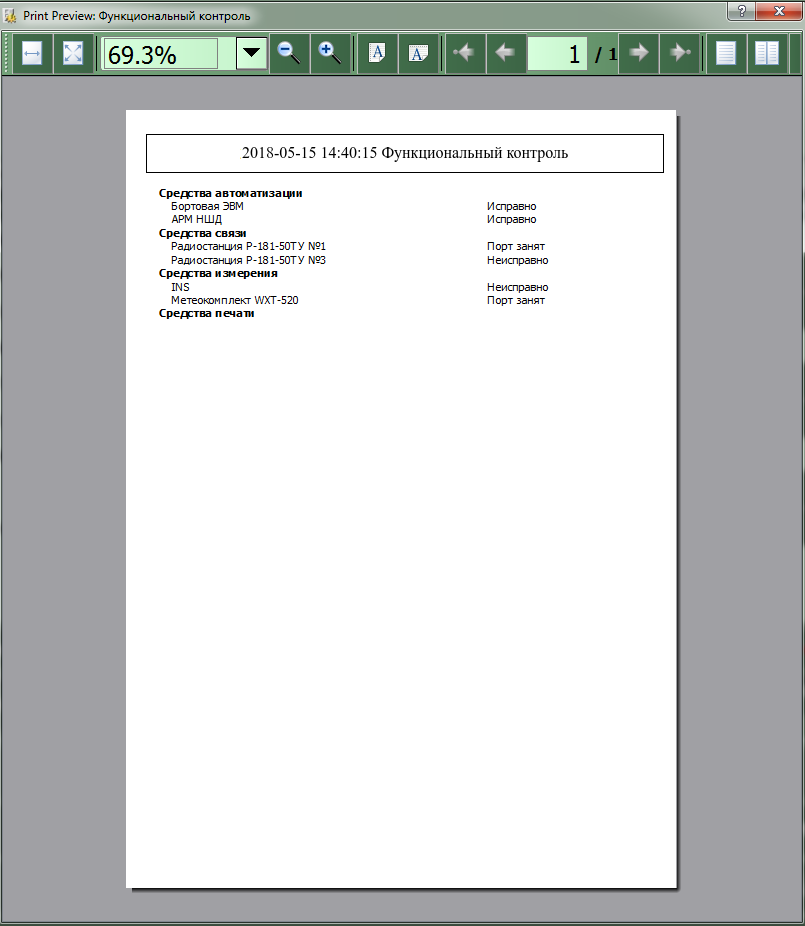
\includegraphics[scale=0.35]{on_print}
	\caption{Окно предварительного просмотра отчета перед печатью}
	\label{fig:guide:user_guide:on_print}
\end{figure}

Программа <<Настройка навигационной системы>> предназначена для настройки бесплатформенной инерциальной навигационной системы БИНС-3.
Для запуска данной системы необходимо запустить файл VSettBINS3.exe.
В результате вызова функции отобразится окно <<Настройка навигационной системы INS>>, приведенное на рис.
\ref{fig:guide:user_guide:ins_window}.
\begin{figure}[!htb]
	\centering
	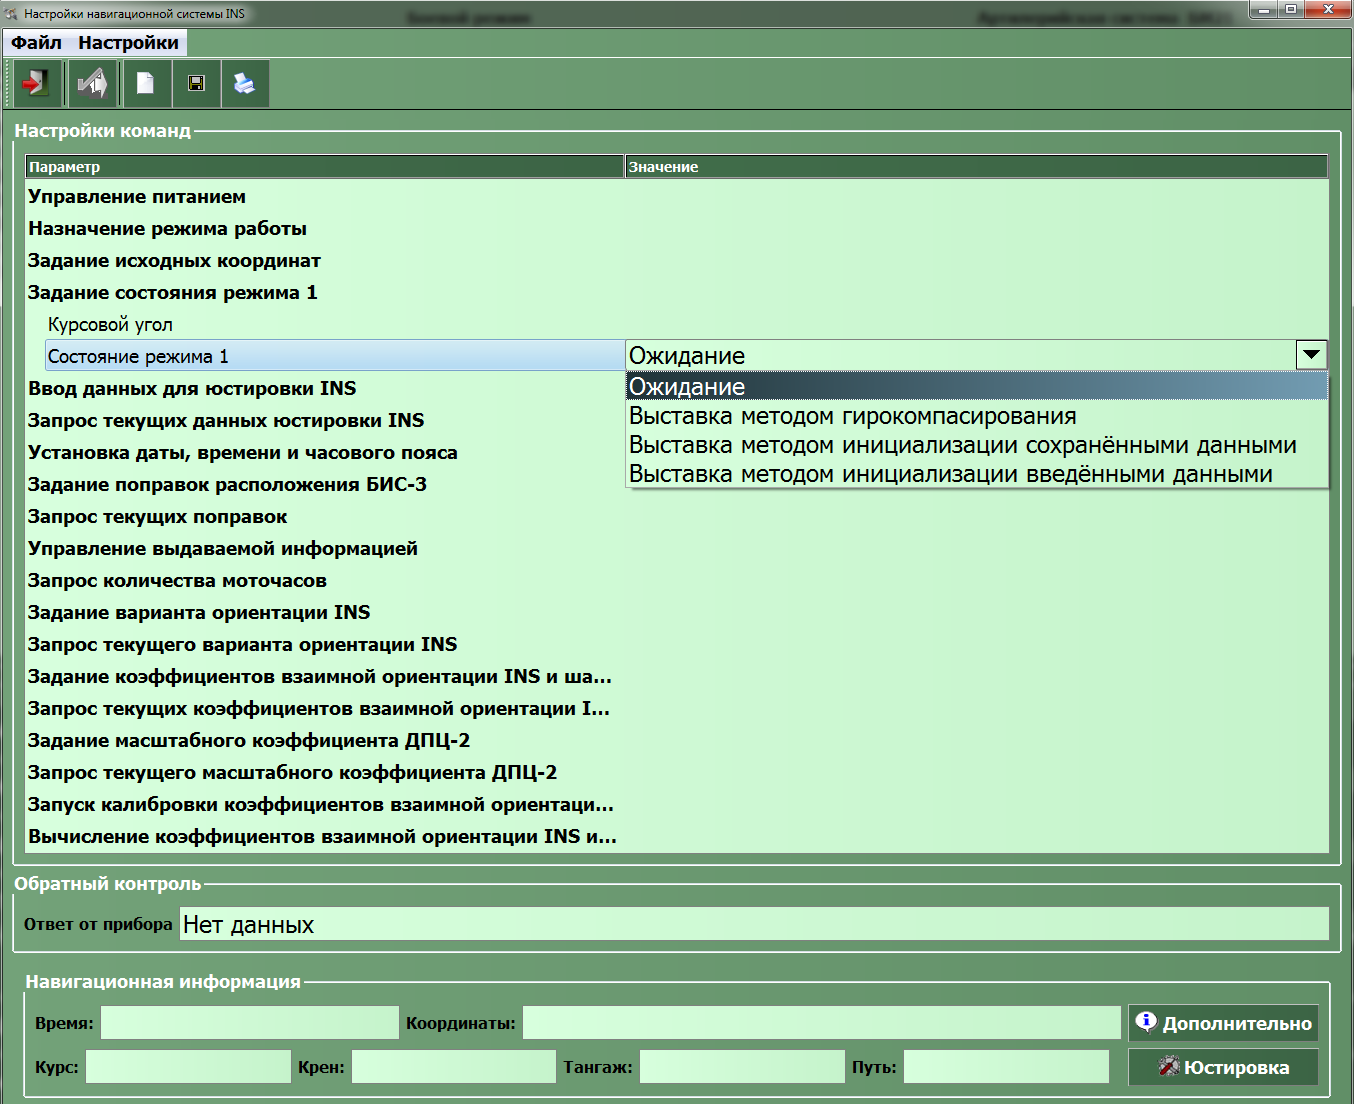
\includegraphics[scale=0.30]{ins_window}
	\caption{Настройка навигационной системы INS}
	\label{fig:guide:user_guide:ins_window}
\end{figure}
В группе <<Навигационная информация>> в полях <<Время>>, <<Координаты>>, <<Курс>>, <<Крен>>, <<Тангаж>>, <<Путь>> спустя некоторое
время после включения будут
отображаться соответствующие данные, полученные в навигационном сообщении от БИНС-3.

При нажатии кнопки <<Юстировка>> (см. рис. \ref{fig:guide:user_guide:ins_window}) отобразится окно для ввода данных,
необходимых при юстировке БИНС-3 (рис. \ref{fig:guide:user_guide:ust}).
Поля <<Курсовой угол>>, <<Крен>>, <<Тангаж>> - редактируемые числовые поля.
После завершения работ по юстировке БИНС-3 закрытие окна осуществляется нажатием на кнопку <<Закрыть>>.
\begin{figure}[!h]
	\centering
	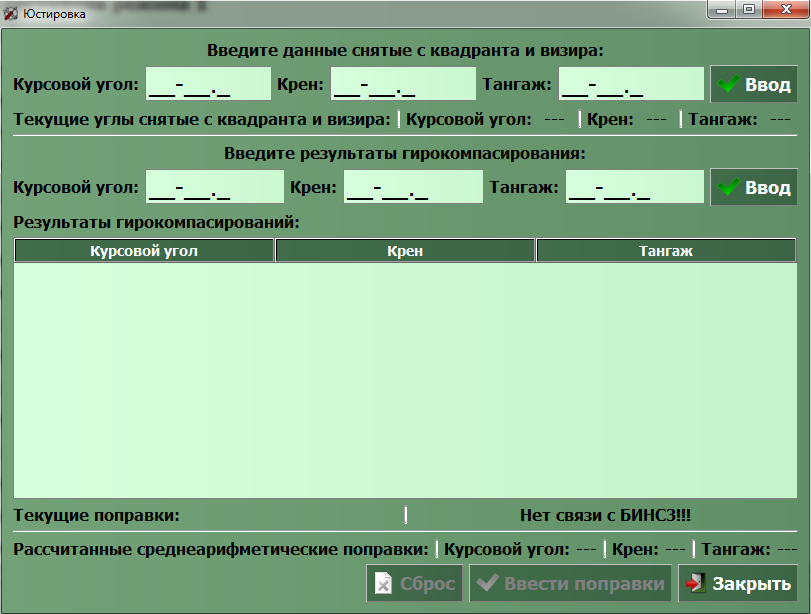
\includegraphics[scale=0.35]{ust}
	\caption{Окно <<Юстировка>>}
	\label{fig:guide:user_guide:ust}
\end{figure}
Для выхода из окна <<Настройка навигационной системы INS>> нажать кнопку <<Выход>> на панели инструментов
или выполнить команду <<Выход>> из меню <<Файл>> (см. рис. \ref{fig:guide:user_guide:ins_window}).

Программа <<Настройка метеостанции WXT-520>> предназначена для настройки настройки метеостанции.
Для запуска данной системы необходимо запустить файл VSetMeteoWXT520.exe.
В результате вызова функции отобразится окно <<Настройка метеостанции WXT-520>>, приведенное на рис.
\ref{fig:guide:user_guide:meteo_window}.
\begin{figure}[!h]
	\centering
	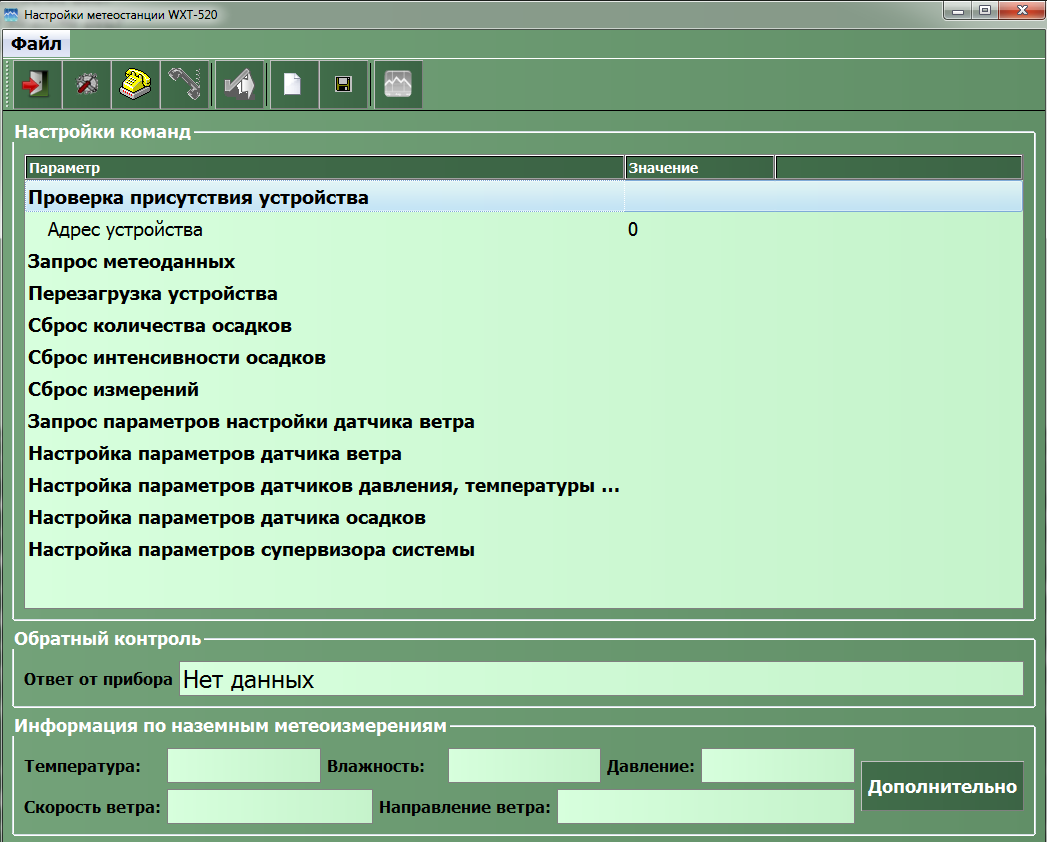
\includegraphics[scale=0.35]{meteo_window}
	\caption{Настройка метеостанции}
	\label{fig:guide:user_guide:meteo_window}
\end{figure}
Если от метеостанции получен ответ, то в поле <<Ответ от прибора>> будет отображаться информация <<Активна>>.

Cлева направо на панели инструментов (см. рис. \ref{fig:guide:user_guide:meteo_window}) расположены\break кнопки: <<Выход>>,
<<Настройки>>, <<Открыть порт>>, <<Закрыть порт>>, <<Отправить сообщение>>, <<Очистить историю сообщений>>,
<<Сохранить историю сообщений>>, <<Сценарий автоматической настройки>>.

В меню <<Файл>> могут выполняться следующие команды:
\begin{itemize}
	\item <<Настройки>>;
	\item <<Открыть порт>>;
	\item <<Основные команды>>;
	\item <<Закрыть порт>>;
	\item <<Полный перечень команд>>;
	\item <<Показать историю сообщений>>;
	\item <<Сохранить историю сообщений>>;
	\item <<Выход>>.
\end{itemize}

Для отправки выбранной команды (по усмотрению оператора) необходимо нажать кнопку <<Отправить сообщение>> на панели инструментов, либо выбрать команду
<<Отправить сообщение>> из контекстного меню. В строке <<Ответ от прибора>> появится ответная информация на выданную команду.
Текущая принятая информация с данными наземных метеоизмерений отображается в соответствующих строках: <<Температура>>,
<<Влажность>>, <<Давление>>, <<Скорость ветра>>, <<Направление ветра>>.


\newcommand{\byr}{руб}

\section{Технико-экономическое обоснование разработки системы функционального контроля технических средств КМУ
артиллерийского дивизиона}

% Begin Calculations
\FPeval{\bonusRate}{1.75}

\FPeval{\leadDevHours}{55}
\FPeval{\devHours}{180}
\FPeval{\qaHours}{120}

\FPeval{\leadDevPerMonth}{2995.5}
\FPeval{\devPerMonth}{1180}
\FPeval{\qaPerMonth}{998.5}

\FPeval{\normativeManHours}{168}

\FPeval{\leadDevPerHourExact}{\leadDevPerMonth / \normativeManHours}
\FPeval{\devPerHourExact}{\devPerMonth / \normativeManHours}
\FPeval{\qaPerHourExact}{\qaPerMonth / \normativeManHours}

\FPround{\leadDevPerHour}{\leadDevPerHourExact}{3}
\FPround{\devPerHour}{\devPerHourExact}{3}
\FPround{\qaPerHour}{\qaPerHourExact}{3}

\FPeval{\leadDevSalaryExact}{\leadDevHours * \leadDevPerHourExact}
\FPeval{\devSalaryExact}{\devHours * \devPerHourExact}
\FPeval{\qaSalaryExact}{\qaHours * \qaPerHourExact}

\FPround{\leadDevSalary}{\leadDevSalaryExact}{1}
\FPround{\devSalary}{\devSalaryExact}{1}
\FPround{\qaSalary}{\qaSalaryExact}{1}

\FPeval{\totalSalaryExact}{clip(\leadDevSalaryExact + \devSalaryExact + \qaSalaryExact) * \bonusRate}

\FPround{\totalSalary}{\totalSalaryExact}{1}

\FPeval{\normExtraSalary}{15}

\FPeval{\extraSalaryExact}{\totalSalaryExact * \normExtraSalary / 100}
\FPround{\extraSalary}{\extraSalaryExact}{1}

\FPeval{\socialFeesCoeff}{34.6}
\FPeval{\socialFeesExact}{clip(\totalSalaryExact + \extraSalaryExact) * \socialFeesCoeff / 100}
\FPround{\socialFees}{\socialFeesExact}{1}

\FPeval{\extraFeesCoeff}{125}
\FPeval{\extraFeesExact}{\totalSalaryExact * \extraFeesCoeff / 100}
\FPround{\extraFees}{\extraFeesExact}{1}

\FPeval{\totalExpensesExact}{\totalSalary + \extraSalary + \socialFees + \extraFees}
\FPround{\totalExpenses}{\totalExpensesExact}{1}

\FPeval{\profitTax}{18}
\FPeval{\ndsNormative}{20}

\FPeval{\productPrice}{21000}

\FPeval{\ndsExact}{clip(\productPrice * \ndsNormative)  / clip(100 + \ndsNormative)}
\FPround{\nds}{\ndsExact}{1}

\FPeval{\cleanProfitDevExact}{\productPrice - \ndsExact - \totalExpensesExact}
\FPround{\cleanProfitDev}{\cleanProfitDevExact}{1}

\FPeval{\cleanProfitExact}{\cleanProfitDevExact - \cleanProfitDevExact * \profitTax / 100}
\FPround{\cleanProfit}{\cleanProfitExact}{1}

\FPeval{\profitLevelExact}{\cleanProfitExact / \totalExpenses * 100}
\FPround{\profitLevel}{\profitLevelExact}{1}

\FPeval{\credit}{8.5}

% End Calculations


\subsection{Описание функций, назначения и потенциальных пользователей ПО}

Система функционального контроля технических средств КМУ артиллерийского дивизиона предназначена для использования в
армейских подразделениях. Данная система используется как часть комплекса автоматизации АРМ артиллерийского дивизиона.

Разработанная система обладает следующими функциями:
\begin{itemize}
		\item тестирование АРМ;
		\item тестирование АВСКУ;
		\item тестирование специального принтера;
		\item тестирование КНС;
		\item тестирования МНСТО;
		\item ведение журнала тестирования.
\end{itemize}

Данный продукт разрабатывается под заказ для вооруженных сил.

\subsection{Расчет на разработку ПО}

Расчет затрат на разработку ПО рассчитывается упрощенно, на основе следующих статей~\cite{economics_diploma}:
\begin{itemize}
	\item затраты на основную заработную плату разработчиков;
	\item затраты на дополнительную заработную плату разработчиков;
	\item отчисления на социальные нужды;
	\item прочие отчисления (амортизационные отчисления, арендная плата за помещения и
		оборудование, расходы на управление и реализацию, расходы на электроэнергию и тому подобное).
\end{itemize}

Произведем расчет данных статей.

\subsubsection{Затраты на основную заработную плату разработчиков}

Затраты на основную заработную плату команды разработчиков определяются исходя из численности и состава команды,
размеров месячной заработной платы каждого из участника команды, а также общей трудоемкости разработки программного
обеспечения.


\begin{equation}
  \label{eq:econ:main_salary}
	\text{З}_\text{о} = \text{К}_\text{пр} \cdot \sum_{i = 1}^{n} \text{З}_\text{чi} \cdot t_{i} \text{\,,}
\end{equation}

\begin{explanation}
	где & $ \text{K}_\text{пр} $ & коэффициент премий; \\
	& $ \text{З}_\text{чi} $ & часовая заработанная плата i-го исполнителя, руб; \\
	& $ t_{i} $ & трудоемкость работ, выполняемых i-м исполнителем, ч; \\
	& $ n $ & количество исполнителей, занятых разработкой конкретного ПО.
\end{explanation}

Часовая заработная плата определяется путем деления месячной заработной платы на количество рабочих часов в месяце и
рассчитывается по формуле~\ref{eq:econ:hour_salary}.

\begin{equation}
  \label{eq:econ:hour_salary}
	\text{З}_\text{чi} = \frac{\text{З}_\text{мi}}{\text{Ф}_\text{рв}} \text{\,,}
\end{equation}

\begin{explanation}
	где & $ \text{З}_\text{мi} $ & месячная заработная плата i-го участника команды, руб; \\
	& $ \text{Ф}_\text{рв} $ & установленный фонд рабочего времени, \num{\normativeManHours} ч.
\end{explanation}

Средняя заработная плата по Республике Беларусь берется из открытого источника~\cite{salaries}.

Расчет затрат на основную заработную плату команды разработчиков приведен в таблице~\ref{table:econ:salaryCalc}.

\begin{table}[!ht]
\small
\caption{Расчет затрат на основную заработную плату команды разработчиков}
	\label{table:econ:salaryCalc}
	\centering
	\begin{tabular}{| >{\centering}m{0.14\textwidth}
		| >{\centering}m{0.17\textwidth}
		  | >{\centering}m{0.13\textwidth}
		  | >{\centering}m{0.12\textwidth}
		  | >{\centering}m{0.15\textwidth}
		  | >{\centering\arraybackslash}m{0.13\textwidth}|}

		\hline
		Участники команды & Вид выполняемой работы & Месячная заработная плата, р. & Часовая заработная плата, р. &
		Трудоемкость работ, ч. & Зарплата по тарифу, р. \\

		\hline
		Ведущий инженер-программист & Разработка архитектуры & \num{\leadDevPerMonth} & \num{\leadDevPerHour} &
		\num{\leadDevHours} & \num{\leadDevSalary} \\

		\hline
		Инженер-программист & Реализация программного продукта & \num{\devPerMonth} & \num{\devPerHour} &
		\num{\devHours} & \num{\devSalary} \\

		\hline
		Тестировщик & Тестирование программного продукта & \num{\qaPerMonth} & \num{\qaPerHour} & \num{\qaHours}
		& \num{\qaSalary} \\

		\hline
		\multicolumn{5}{|l|}{Премия} & \num{\bonusRate} \\

		\hline
		\multicolumn{5}{|l|}{Итого затраты на основную заработную плату разработчиков} & \num{\totalSalary} \\
		\hline
	\end{tabular}
\end{table}

\subsubsection{Затраты на дополнительную заработную плату разработчиков}

Данные затраты включают в себя выплаты, предусмотренные законодательством о труде:
\begin{itemize}
	\item оплата льготных часов;
	\item оплата времени выполнения государственных обязанностей;
	\item оплаты трудовых отпусков;
	\item выплаты, не связанные с основной деятельностью исполнителей.
\end{itemize}

Затраты на дополнительную заработную плату разработчиков определяются по следующей формуле

\begin{equation}
  \label{eq:econ:extra_salary}
	\text{З}_\text{д} = \frac{\text{З}_\text{о} \cdot \text{Н}_\text{д}}{\num{100}} \text{\,,}
\end{equation}

\begin{explanation}
	где & $ \text{З}_\text{о} $ & затраты на основную заработную плату, руб; \\
	& $ \text{Н}_\text{д} $ & норматив дополнительной заработной платы, \num{\normExtraSalary} \%.
\end{explanation}

Зарплаты на дополнительную заработную плату:

\begin{equation}
  \label{eq:econ:extra_salary_calc}
	\text{З}_\text{д} = \frac{\num{\totalSalary} \cdot \num{\normExtraSalary}}{\num{100}} = \num{\extraSalary} {\text{ \byr}} \text{.}
\end{equation}

\subsubsection{Отчисления на социальные нужды}

Отчисления на социальные нужды идут в фонд социальной защиты населения и на обязательное страхование. Эти отчисления определяются в соответствии с действующими законодательными актами по формуле

\begin{equation}
  \label{eq:econ:social_fees}
	\text{Р}_\text{соц} = \frac{(\text{З}_\text{о} + \text{З}_\text{д}) \cdot \text{Н}_\text{соц}} {\num{100}} \text{\,,}
\end{equation}

\begin{explanation}
	где & $ \text{Н}_\text{соц} $ & норматив отчислений на социальные нужды, \num{\socialFeesCoeff} \%.
\end{explanation}

Отчисления на социальные нужды:

\begin{equation}
  \label{eq:econ:social_fees_calc}
	\text{З}_\text{о} = \frac{(\num{\totalSalary} + \num{\extraSalary}) \cdot \num{\socialFeesCoeff}}{\num{100}} =
	\num{\socialFees} {\text{ \byr}} \text{.}
\end{equation}

\subsection{Прочие отчисления}

Прочие затраты включаются в себестоимость разработки ПО в процентах от затрат на основную заработную плату команды
разработчиков.

\begin{equation}
  \label{eq:econ:extra_fees}
	\text{З}_\text{пз} = \frac{\text{З}_\text{о} \cdot \text{Н}_\text{пз}} {\num{100}} \text{\,,}
\end{equation}

\begin{explanation}
	где & $ \text{Н}_\text{пз} $ & норматив прочих затрат, \num{\extraFeesCoeff} \%.
\end{explanation}

Прочие затраты составляют:

\begin{equation}
  \label{eq:econ:extra_fees_calc}
	\text{З}_\text{пз} = \frac{\num{\totalSalary} \cdot \num{\socialFeesCoeff}}{\num{100}} =
	\num{\extraFees} {\text{ \byr}} \text{.}
\end{equation}

\subsection{Полная сумма затрат}
Полная сумма затрат на разработку программного обеспечения находится путем суммирования всех рассчитанных статей затрат

\begin{table}[!ht]
	\caption{Затраты на разработку программного обеспечения}
	\label{table:econ:total_expenses}
	\centering
	\begin{tabular}{| >{\raggedright}m{0.82\textwidth}
		  | >{\centering\arraybackslash}m{0.13\textwidth}|}

		\hline
		\centering{Статья затрат} & Сумма, р. \\

		\hline
		Основная заработная плата команды разработчиков & \num{\totalSalary} \\

		\hline
		Дополнительная заработная плата команды разработчиков & \num{\extraSalary} \\

		\hline
		Отчисления на социальные нужды & \num{\socialFees} \\

		\hline
		Прочие затраты & \num{\extraFees} \\

		\hline
		Общая сумма затрат на разработку & \num{\totalExpenses} \\

		\hline
	\end{tabular}
\end{table}

\subsection{Оценка результата разработки и использования ПО}

При разработке или использовании программного продукта можно получить экономический эффект, который напрямую влияет
на экономические показатели компании, или неэкономический эффект, который напрямую не связан с экономическими
показателями деятельности компании.

\subsection{Экономический эффект}

При разработке программного обеспечения под заказ экономический эффект может быть рассчитан как для
организации-разработчика, так и для заказчика ПО. В нашем случае, экономический эффект получает только\break организация-разработчик.

Экономическим эффектом для организации-разработчика является чистая прибыль,
если организация является плательщиком налогов, либо прибыль до налогообложения, если организация освобождена от уплаты
налогов на прибыль, полученная от реализации программного обеспечения.
В нашем случае, компания является налогоплательщиком, следовательно, нужно рассчитать чистую прибыль.

Чистая прибыль для организаций, которые являются плательщиком налога на прибыль, рассчитывается по формуле

\begin{equation}
  \label{eq:econ:clean_profit}
	\text{П}_\text{ч} = \text{П} - \frac{\text{П} \cdot \text{Н}_\text{п}} {\num{100}} \text{\,,}
\end{equation}

\begin{explanation}
	где & $ \text{П} $ & прибыль до налогообложения, руб; \\
	& $ \text{Н}_\text{п} $ & ставка налога на прибыль, в соответствии с действующим законодательством,
	\num{\profitTax}\%.
\end{explanation}

Прибыль до налогообложения организации-разработчика рассчитывается по формуле

\begin{equation}
  \label{eq:econ:clean_profit_dev}
	\text{П} = \text{Ц} - \text{НДС} - \text{З}_\text{р} \text{\,,}
\end{equation}

\begin{explanation}
	где & $ \text{Ц} $ & цена реализации программного продукта заказчику, руб; \\
	& $ \text{НДС} $ & сумма налога на добавленную стоимость, руб; \\
	& $ \text{З}_\text{р} $ & затраты на разработку программного обеспечения, руб.
\end{explanation}

Сумма налога на добавленную стоимость рассчитывается для организаций, являющимися плательщиками НДС,
по следующей формуле

\begin{equation}
  \label{eq:econ:nds}
  \text{НДС} =
    \frac{ \text{Ц} \cdot \text{Н}_{\text{дс}} }
	 { \num{100}\text{\%} + \text{Н}_\text{дс} } \text{\,,}
\end{equation}

\begin{explanation}
	где & $ \text{Н}_{\text{дс}} $ & ставка налога на добавленную стоимость согласно действующему законодательству,
	\num{\ndsNormative}\%.
\end{explanation}

Цена программного продукта устанавливается на основе цен на программное обеспечение, выполняющие схожие функции.
Для данного продукта отсутствуют точные аналоги в открытом доступе, поэтому цена формировалась на основе нескольких
продуктов, предлагающих похожий функционал. В результате была установлена цена в размере \num{\productPrice} руб.

Сумма налога на добавленную стоимость составляет:

\begin{equation}
  \label{eq:econ:nds_calc}
  \text{НДС} =
	\frac{ \num{\productPrice} \cdot \num{\ndsNormative}}
	 { \num{100} + \num{\ndsNormative}} = \num{\nds} \text{ \byr.}
\end{equation}

Прибыль до налогообложения составляет:
\begin{equation}
  \label{eq:econ:clean_profit_dev_calc}
	\text{П} = \num{\productPrice} - \num{\nds} - \num{\totalExpenses}
	 = \num{\cleanProfit} \text{ \byr.}
\end{equation}

Экономический эффект с учетом налога на прибыль, рассчитанный по формуле~\ref{eq:econ:clean_profit}:
\begin{equation}
  \label{eq:econ:clean_profit_calc}
	\text{П}_\text{ч} = \num{\cleanProfitDev} - \frac{\num{\cleanProfitDev} \cdot \num{\profitTax}}{\num{100}}
	 = \num{\cleanProfit} \text{ \byr.}
\end{equation}

Для того, чтобы сделать вывод об эффективности разработки и реализации программного продукта по установленной цене,
необходимо рассчитать уровень рентабельности.
Рассчитанный уровень рентабельности сравнивается со средней ставкой по банковским депозитам.

Уровень рентабельности рассчитывается по формуле
\begin{equation}
  \label{eq:econ:profit_level}
	\text{У}_\text{р} =
	\frac{\text{П}_\text{ч}}
	 {\text{З}_\text{р}} \cdot \num{100}{\text{\%}} \text{.}
\end{equation}

Уровень рентабельности составляет
\begin{equation}
  \label{eq:econ:profit_level_calc}
	\text{У}_\text{р} = \frac{\num{\cleanProfit}}{\num{\totalExpenses}} \cdot \num{100}\text{\%}
	 = \num{\profitLevel} \text{ \%.}
\end{equation}

Средняя ставка по банковским депозитам на апрель месяц для юридических лиц составляет \num{\credit}\%.
Сравнивая уровень рентабельности и среднюю ставку по банковским депозитам можно сделать вывод,
что проект экономически эффективен, т.к. уровень рентабельности больше, чем средняя ставка по банковским депозитам.

\subsection{Неэкономический эффект}

Для организации-заказчика данный продукт приводит к получению\break только неэкономического эффекта.
При использовании данного программного продукта в составе комплекса автоматизации АРМ, с офицеров снимаются задачи по
обнаружению и настройке подключенных устройств вручную, упрощается процесс тестирования и мониторинга подключенных
\break
устройств.

\hfill
\clearpage




\sectioncentered*{Заключение}
\addcontentsline{toc}{section}{Заключение}

В ходе дипломного проектирования было изучено множество литературных источников, относящихся к предметной области. Было
проведено исследование наиболее близких к системе аналогов и обзор технических\break средств, тестирование которых необходимо
реализовать. В результате исследования аналогов прямых аналогов разрабатываемой системы не было выявлено.

В процессе разработки были детально изучены протоколы взаимодействия устройств с ЭВМ, также были исследованы особенности
работы и применения данных устройств. Полученная информация выявила необходимость подключения как устройств,
подключенных посредством ЛВС, так и\break устройств, подключенных непосредственно к портам ЭВМ через COM порты.

В ходе анализа технических средств, тестирование которых необходимо реализовать, в архитектуре приложения было
принято решение использовать модульных подход. Выбор данного подхода обусловлен тем, что подключаемые к ЭВМ
устройства не зависят друг от друга. Данный подход позволил создать масштабируемую архитектуру, обеспечивающую простую
интеграцию новых модулей в систему.

В процессе работы над проектом были разработаны и описаны следующие схемы:
\begin{itemize}
	\item структурная схема;
	\item диаграмма последовательности;
	\item схема программы, описывающая процесс тестирования устройств;
	\item схема программы, описывающая процесс тестирования БИНС.
\end{itemize}

В процессе разработки была реализована программы настройки и тестирования устройств.
Также была реализована программа для работы с журналом тестирования. Было приведено технико-экономическое обоснование
целесообразности производства системы.

В результате была разработана система, обладающая следующими возможностями:
\begin{itemize}
	\item тестирование подключенных устройств;
	\item журналирование;
	\item настройка технических средств.
\end{itemize}

Данная система обладает следующими достоинствами:
\begin{itemize}
	\item масштабируемость;
	\item простота;
	\item многофункциональность.
\end{itemize}

Разработанный проект может быть использован для интеграции в системы автоматизации КМУ артиллерийского дивизиона.



% Зачем: Изменение надписи для списка литературы
% Почему: Пункт 2.8.1 Требований по оформлению пояснительной записки.
\renewcommand{\bibsection}{\sectioncentered*{Cписок использованных источников}}
\phantomsection\pagebreak% исправляет нумерацию в документе и исправляет гиперссылки в pdf
\addcontentsline{toc}{section}{Cписок использованных источников}

% Зачем: Печать списка литературы. База данных литературы - файл bibliography_database.bib
\bibliography{bibliography_database}


\setminted[c++]{fontfamily=tt,fontsize=\scriptsize,xleftmargin=0ex,breaklines=true,tabsize=4}
\sectionadd*{ПРИЛОЖЕНИЕ А}
\addcontentsline{toc}{appendix}{ПРИЛОЖЕНИЕ А. Листинг кода класса \texttt{OffLineFuncControl}}
\label{sec:appendix_a}


\begin{center}
	\normalfont\normalsize{\textit{(обязательное)}}

	\normalfont\normalsize{Листинг кода класса \texttt{OffLineFuncControl}}
\end{center}


\begin{minted}{c++}
#include "OffLineFuncControl.h"
#include <QPixmap>
#include <QBitmap>
#include <QMessageBox>
#include <QFont>
#include <QFile>
#include <QDir>
#include <QActionGroup>
#include <QCheckBox>
#include <QMessageBox>
#include <QByteArray>
#include <QTreeWidgetItem>
#include <QTreeWidgetItemIterator>
#include <QtTest/QtTest>
#include <QTextStream>
#include <QHostAddress>
#include "Fun.h"
#include "RusTextFunkControl.h"
#include "RusTextRedUsers.h"
#include "QTestPrinter.h"
#include "QTestARM.h"
#include "VTest_R181.h"
#include "VTest_MeteoWXT520.h"
#include "VTest_1D22.h"
#include "VTest_BI.h"
#include "VTest_BINS3.h"
#include "CoordContain.h"
#include "VTest_GPS.h"
#include "VTest_Kaponir.h"

#include "Journal.h"


#include <QPrintPreviewDialog>
#include <QPainter>
#include <QFont>
#include <QDateTime>
#include <QCalendarWidget>
#include <QDialog>
#include <QGridLayout>
#include <QDateEdit>
#include <QTimeEdit>
#include <QDateTimeEdit>
#include <QProcess>
#include <QStatusBar>
#include "VPushButtonIdent.h"

#include "StaticGlobalFunc.h"
#include "qdbloader.h"
#include "qtsingleapplication.h"

#define CR "<br />"

OffLineFuncControl::OffLineFuncControl(QWidget *parent, Qt::WFlags flags)
	: QMainWindow(parent, flags)
{

	QDir dir = QDir::current();
	if (dir.cdUp()) {
		QString sDir = dir.absolutePath();
		QFile file(sDir + "/StyleSheet/ScreenStyleLegion.stl");
		if (file.open(QIODevice::ReadOnly)) {
			QByteArray s = file.readAll();
			QString sStyle(s);
			qApp->setStyleSheet(sStyle);
			m_Menu.setStyleSheet(sStyle);
			file.close();
		}
	}
	QString sTimeCompile = __TIMESTAMP__;
	QDateTime tt = QDateTime::fromString(sTimeCompile);

	m_sockReceiveUpdate.bind(QHostAddress::LocalHost, 15558, QUdpSocket::ReuseAddressHint);

	m_pActInfo = m_Menu.addAction(QIcon(":/OffLineFuncControl/Resources/info.png"), ID_FUNC_FONE_4);

	m_pActSetParam = m_Menu.addAction(ID_FUNC_FONE_5);
	m_pMenuSNS = m_Menu.addMenu(tr("Выбор СНС"));
	m_pActSNS_GPS_GLONASS = m_pMenuSNS->addAction(tr("GPS/Глонасс"));
	m_pActSNS_GPS = m_pMenuSNS->addAction(tr("GPS"));
	m_pActSNS_GLONASS = m_pMenuSNS->addAction(tr("Глонасс"));
	QActionGroup * pActGr = new QActionGroup(this);
	pActGr->addAction(m_pActSNS_GPS_GLONASS);
	pActGr->addAction(m_pActSNS_GPS);
	pActGr->addAction(m_pActSNS_GLONASS);

	m_bStartTest = false;
	setMinimumSize(800, 450);
	QWidget * pCentralWidg = new QWidget(this);
	setCentralWidget(pCentralWidg);

	setWindowTitle(ID_FUNC1);

	QPixmap picFunControl = QPixmap(":/OffLineFuncControl/Resources/fun_control.PNG");
	picFunControl.setMask(picFunControl.createHeuristicMask());
	setWindowIcon(QIcon(picFunControl));

	m_pTreeDevice = new QSimpleBWTree(pCentralWidg);
	m_pTreeDevice->setRootIsDecorated(true);
	m_pTreeDevice->setColumnCount(3);
	m_pTreeDevice->setColumnForSelect(1);
	m_pTreeDevice->setHeaderLabels(QStringList() << ID_FUNC_AKPP_1 << ID_FUNC_AKPP_2 << tr("Информация"));
	QTreeWidgetItem * pHeader = m_pTreeDevice->headerItem();

	if (pHeader) {
		pHeader->setSizeHint(0, QSize(0, 32));
	}

	m_pBtStart = new QPushButton(ID_FUNC12, pCentralWidg);
	m_pBtStart->setIcon(QIcon(":/OffLineFuncControl/Resources/play.png"));
	m_pBtStart->setObjectName("pbCentred");

	m_pBtPrint = new QPushButton(tr("Печать"), pCentralWidg);
	m_pBtPrint->setIcon(QIcon(":/OffLineFuncControl/Resources/print.png"));
	m_pBtPrint->setObjectName("pbCentred");

	m_pBtSettings = new QPushButton(ID_FUNC3, pCentralWidg);
	m_pBtSettings->setIcon(QIcon(":/OffLineFuncControl/Resources/nastr_ARM.PNG"));
	m_pBtSettings->setObjectName("pbCentred");

	m_pBtJournal = new QPushButton(ID_FUNK_JOURNAL_OPEN, pCentralWidg);
	m_pBtJournal->setIcon(QIcon(":/OffLineFuncControl/Resources/marshruty.PNG"));
	m_pBtJournal->setObjectName("pbCentred");

	m_pBtTestKS = new QPushButton(tr("Тест КС"), pCentralWidg);
	m_pBtTestKS->setIcon(QIcon(":/OffLineFuncControl/Resources/Radio.png"));
	m_pBtTestKS->setObjectName("pbCentred");

	m_pBtExit = new QPushButton(tr("Закрыть"), pCentralWidg);
	m_pBtExit->setIcon(QIcon(":/OffLineFuncControl/Resources/Exit.PNG"));

	loadDevices();

	connect(m_pTreeDevice, SIGNAL(itemClicked(QTreeWidgetItem *, int)), this, SLOT(onChangeCheckDevice(QTreeWidgetItem *, int)));
	connect(m_pTreeDevice, SIGNAL(keyPress(int)), this, SLOT(onChangeCheckDevice(int)));
	connect(m_pTreeDevice, SIGNAL(signCustomContextMenu(QPoint &)), this, SLOT(onMenu(QPoint &)));
	connect(m_pActInfo, SIGNAL(triggered()), this, SLOT(onInfo()));
	connect(m_pBtStart, SIGNAL(clicked()), this, SLOT(onStart()));
	connect(m_pBtPrint, SIGNAL(clicked()), this, SLOT(onPrint()));
	connect(m_pBtJournal, SIGNAL(clicked()), this, SLOT(onJournal()));
	connect(m_pBtSettings, SIGNAL(clicked()), this, SLOT(onSettings()));
	connect(m_pBtTestKS, SIGNAL(clicked()), this, SLOT(onTestKS()));
	connect(m_pBtExit, SIGNAL(clicked()), this, SLOT(close()));
	connect(&m_sockReceiveUpdate, SIGNAL(readyRead()), SLOT(receiveSignalUpdate()));
}

OffLineFuncControl::~OffLineFuncControl()
{

}

void OffLineFuncControl::closeEvent(QCloseEvent * e)
{
	QtSingleApplication * pApp =   qobject_cast<QtSingleApplication *>(qApp);
	if (pApp)
	{
		pApp->sendMessage("Imitator_R181", "LEGIONPANEL:TERMINATE");
	}

	e->accept();
}

void OffLineFuncControl::receiveSignalUpdate()
{
	while (m_sockReceiveUpdate.hasPendingDatagrams())
	{
		QByteArray datagram;
		datagram.resize(m_sockReceiveUpdate.pendingDatagramSize());
		QHostAddress sender;
		quint16 senderPort;

		m_sockReceiveUpdate.readDatagram(datagram.data(), datagram.size(),
				&sender, &senderPort);

		loadDevices();
	}
}

void OffLineFuncControl::onInfoDevice(QVariant id)
{
	QTreeWidgetItem * item = m_pTreeDevice->findItemByDataUnique(1, id);

	if (!item)
		return;

	QString sInfo = item->data(2, Qt::UserRole).toString();

	QDialog dlg(m_pTreeDevice);
	QTextEdit textInfo(&dlg);
	QPushButton btExit(&dlg);
	btExit.setText(tr("Закрыть"));
	QGridLayout l(&dlg);
	l.addWidget(&textInfo);
	l.addWidget(&btExit);
	connect(&btExit, SIGNAL(clicked()), &dlg, SLOT(accept()));

	dlg.setWindowTitle(ID_FUNC_FONE_4 + ": " + item->text(0));
	dlg.setMinimumWidth(350);
	dlg.resize(700, 600);
	textInfo.setReadOnly(true);

	textInfo.setHtml (sInfo);
	dlg.exec();
}

void OffLineFuncControl::onInfo()
{
	QTreeWidgetItem * item = m_pTreeDevice->currentItem();
	if (!item)
		return;
	QTreeWidgetItem * itemParent = item->parent();
	if (!itemParent)
		return;

	QVariant idDevice = item->data(1, Qt::UserRole);

	onInfoDevice(idDevice);


}

quint8 OffLineFuncControl::onTestARM(quint8 numARM, QString & sRez) {

	if ((numARM >= 1 && numARM <= 4) || numARM == 7) {
		QTestARM test(this);
		return test.test(numARM, sRez);
	}


	return 3;
}

void OffLineFuncControl::messageReceived(const QString& message)
{
	if (message == "OffLineFuncControl" || message == "LEGIONPANEL:ACTIVATE")
	{
		QRect r = geometry();
		this->hide();
		this->setWindowState(Qt::WindowMinimized);
		this->setVisible(true);
		this->setWindowState(this->windowState() & ~Qt::WindowMinimized | Qt::WindowActive);

		this->raise();
		this->activateWindow();
		setGeometry(r);
	}
	else if (message == "UPDATE_SETT_ARM")
	{
	}
	else if (message == "LEGIONPANEL:TERMINATE")
	{
		close();
	}

}


void OffLineFuncControl::onMenu(QPoint & pos) {
	m_pActInfo->setEnabled(true);

	QTreeWidgetItem * item = m_pTreeDevice->currentItem();
	if (!item)
		return;
	if (item->childCount())
		return;
	QString sInfo = item->data(2, Qt::UserRole).toString();
	if (!sInfo.length())
		m_pActInfo->setEnabled(false);


	quint8 deviceId = item->data(1, Qt::UserRole).toUInt();



	if ((deviceId == 99)
			&& !m_bStartTest)
	{
		m_pActSetParam->setVisible(true);
		m_pMenuSNS->menuAction()->setVisible(true);
	}
	else
	{
		m_pActSetParam->setVisible(false);
		m_pMenuSNS->menuAction()->setVisible(false);
	}

	m_Menu.popup(pos);

}

void OffLineFuncControl::onStart() {
	if (m_bStartTest)
		return;
	m_bStartTest = true;
	m_pBtStart->setEnabled(false);
	m_pBtPrint->setEnabled(false);
	m_pBtSettings->setEnabled(false);
	m_pBtJournal->setEnabled(false);
	QTreeWidgetItemIterator it(m_pTreeDevice);

	JournalEntry journalEntry;
	QString sRez;
	while (*it) {
		sRez = "";
		QTreeWidgetItem * item = *it;
		if ((item->checkState(0) != Qt::Checked) || item->childCount() || item->isHidden())
		{
			++it;
			continue;
		}

		item->setForeground(1, QBrush(Qt::black));
		item->setText(1, ID_FUNC_FONE_2 + "...");

		quint32 idItem = item->data(1, Qt::UserRole).toUInt();

		m_pTreeDevice->clearSelections();
		m_pTreeDevice->selectItemById(idItem, true);

		QTest::qWait(500);

		QString sNameDevise = item->text(0);
		QString sNameDeviseParent = item->text(0);

		quint8 deviceId = item->data(1, Qt::UserRole).toUInt();

		quint8 rez = 0;

		switch (deviceId)
		{
			case 1:
			case 2:
			case 3:
			case 4:
			case 5:
			case 20:
			case 21:
			case 22:
			case 23:
				{
					///АРМы
					QTestARM test(this);
					rez = test.test(deviceId, sRez);
					break;
				}
			case 6:
			case 7:
			case 8:
			case 9:
			case 109:
			case 10:
			case 16:
				{
					//Р-180, Р-181
					VTest_R181 test(this);
					rez = test.test(deviceId, sRez);
					break;
				}
			case 11:
				{
					//Метеостанция
					VTest_MeteoWXT520 test(this);
					rez = test.test(sRez);
					break;

				}
			case 12:
				{
					//БИНС-3
					VTest_BINS3 test(this);
					rez = test.test(sRez);
					break;

				}
			case 13:
				{
					//1Д22
					VTest_1D22 test(this);
					rez = test.test(sRez);
					break;

				}
			case 14:
				{
					//Капонир
					VTest_Kaponir test(this);
					rez = test.test(sRez);
					break;

				}
			case 15:
				{
					//Блок индикации
					VTest_BI test(this);
					rez = test.test(sRez);
					break;

				}
			case 17:
				{
					//GPS
					VTest_GPS test(this);
					rez = test.test(sRez);
					break;
				}
			case 18:
				{
					//Принтер
					QTestPrinter test(this);
					rez = test.test(sRez);
					break;
				}
		}

		DeviceInfo deviceInfo;
		deviceInfo.deviceName = sNameDevise;
		QString sRezSaved = sRez;
		sRezSaved.replace("\r\n", CR);
		sRezSaved.replace("\"", "\\\"");
		deviceInfo.additionalInfo = sRezSaved;

		item->setData(2, Qt::UserRole, sRez);
		VPushButtonIdent * bt = qobject_cast<VPushButtonIdent *>(m_pTreeDevice->itemWidget(item, 2));
		if (bt)
		{
			bt->setEnabled(sRez.length());
		}
		if (rez == 0)
		{
			item->setForeground(1, QBrush(QColor(0, 150, 0)));
			item->setText(1, ID_FUNC_AKPP_7);
			deviceInfo.resultMessage = ID_FUNC_AKPP_7;
			deviceInfo.hasError = false;
		}
		else if (rez == 1 || rez > 3)
		{
			item->setForeground(1, QBrush(QColor(150, 0, 0)));
			item->setText(1, ID_FUNC_AKPP_8);
			deviceInfo.resultMessage = ID_FUNC_AKPP_8;
			deviceInfo.hasError = true;
		}
		else if (rez == 2)
		{
			item->setForeground(1, QBrush(QColor(150, 0, 0)));
			item->setText(1, ID_FUNC_AKPP_9);
			deviceInfo.resultMessage = ID_FUNC_AKPP_9;
			deviceInfo.hasError = true;
		}
		else if (rez == 3)
		{
			item->setForeground(1, QBrush(QColor(150, 0, 0)));
			item->setText(1, ID_FUNC_AKPP_10);
			deviceInfo.resultMessage = ID_FUNC_AKPP_10;
			deviceInfo.hasError = true;
		}

		saveRezTest(sNameDevise, deviceInfo.resultMessage, rez);

		journalEntry.addDevice(deviceInfo);
		++it;
	}

	Journal::store(journalEntry);

	m_pTreeDevice->clearSelections();
	m_pBtStart->setEnabled(true);
	m_pBtPrint->setEnabled(true);
	m_pBtSettings->setEnabled(true);
	m_pBtJournal->setEnabled(true);
	m_bStartTest = false;

}

bool OffLineFuncControl::saveRezTest(QString sNameDevice, QString sRezSaved, quint8 rez)
{
	QString sDir = QApplication::applicationDirPath();
	QFile f(sDir + "/Journal/data/Last/" + sNameDevice + ".test");

	if (!f.open(QIODevice::ReadWrite))
		return false;

	QTextStream s(&f);
	if (rez)
		s << "0\r\n";
	else
		s << "1\r\n";
	s << sRezSaved;

	f.close();

	return true;
}

void OffLineFuncControl::onChangeCheckDevice(QTreeWidgetItem * item, int column) {
	if (column != 0)
		return;

	if (!item)
		return;

	Qt::CheckState stateOld = (Qt::CheckState)item->data(0, Qt::UserRole).toInt();
	Qt::CheckState state = item->checkState(0);

	item->setData(0, Qt::UserRole, state);

	if (stateOld == state)
		return;

	if (item->childCount() > 0) {

		for (quint32 i = 0; i < item->childCount(); i++) {
			QTreeWidgetItem * itemChild = item->child(i);
			if (!itemChild)
				continue;
			if (!(itemChild->flags() & Qt::ItemIsEnabled))
				continue;
			QString sText = itemChild->text(0);
			itemChild->setCheckState(0, state);

			if (itemChild->childCount() > 0)
				onChangeCheckDevice(itemChild, column);

			itemChild->setData(0, Qt::UserRole, state);

		}
	}

	{
		QTreeWidgetItem * itemParent = item->parent();
		if (!itemParent)
			return;
		if (state == Qt::Checked) {
			itemParent->setCheckState(0, state);
			itemParent->setData(0, Qt::UserRole, state);

			if (itemParent->parent()) {
				itemParent->parent()->setCheckState(0, state);
				itemParent->parent()->setData(0, Qt::UserRole, state);
			}
		} else {
			bool b = true;
			for (quint32 i = 0; i < itemParent->childCount(); i++) {
				QTreeWidgetItem * itemChild = itemParent->child(i);
				if (!itemChild)
					continue;
				if (!(itemChild->flags() & Qt::ItemIsEnabled))
					continue;
				Qt::CheckState st = itemChild->checkState(0);
				if (st == Qt::Checked) {
					b = false;
					break;
				}
			}
			if (b) {
				itemParent->setCheckState(0, Qt::Unchecked);

				if (itemParent->parent()) {
					onChangeCheckDevice(itemParent, column);
				}

				itemParent->setData(0, Qt::UserRole, Qt::Unchecked);
			}

		}

	}

}

void OffLineFuncControl::onChangeCheckDevice(int key) {
	QTreeWidgetItem * pItem = m_pTreeDevice->currentItem();

	if (!pItem)
		return;
	if (key != Qt::Key_Space)
		return;

	onChangeCheckDevice(pItem, 0);

}

void OffLineFuncControl::loadDevices() {

	m_pTreeDevice->clear();

	QList<quint8> groups = getListGroupsDevices();
	QHash<quint8, QTreeWidgetItem *> groupWidgetHash;

	for (quint8 i = 0; i < groups.size(); i++) {

		QTreeWidgetItem * pItemGroup = new QTreeWidgetItem(m_pTreeDevice);
		quint8 groupId = groups[i];
		groupWidgetHash.insert(groupId, pItemGroup);
		QString groupName = getNameGroupDevice( groups[i] );

		QFont f = pItemGroup->font(0);
		f.setBold(true);
		pItemGroup->setFont(0, f);
		pItemGroup->setText(0, groupName);
		pItemGroup->setSizeHint(0, QSize(0, 32));
		m_pTreeDevice->insertTopLevelItem(0, pItemGroup);
		pItemGroup->setExpanded(true);
		Qt::ItemFlags flags = pItemGroup->flags();
		flags |= Qt::ItemIsUserCheckable;

		pItemGroup->setFlags(flags);
		pItemGroup->setCheckState(0, Qt::Checked);
		pItemGroup->setData(0, Qt::UserRole, Qt::Checked);
		pItemGroup->setData(1, Qt::UserRole, 0);

		pItemGroup->setHidden(true);

	}
	_SETT_ARM sett;
	getSettARM(sett);

	QHash<quint8, _IP_DEVICE>& lanDevices =  sett.shemeLAN;
	QHash<quint8, _IP_DEVICE>::iterator lanDeviceIter;
	for (lanDeviceIter = lanDevices.begin(); lanDeviceIter != lanDevices.end(); ++lanDeviceIter)
	{
		quint8 lanDeviceId = lanDeviceIter.key();
		QString lanDeviceName = getNameDevice(lanDeviceId);

		quint8 lanDeviceGroupId = getIdGroupForDevice(lanDeviceId);
		QTreeWidgetItem * groupWidget = groupWidgetHash[lanDeviceGroupId];

		if (!groupWidget)
			continue;

		groupWidget->setHidden(false);

		QTreeWidgetItem * pItem = new QTreeWidgetItem(groupWidget);
		Qt::ItemFlags flags = pItem->flags();
		flags |= Qt::ItemIsUserCheckable;
		pItem->setText(0, lanDeviceName);
		pItem->setFlags(flags);
		pItem->setCheckState(0, Qt::Checked);
		pItem->setData(0, Qt::UserRole, Qt::Checked);
		pItem->setData(1, Qt::UserRole, lanDeviceId);
		pItem->setSizeHint(0, QSize(0, 32));

		QString qstr;
		VPushButtonIdent * pBtInfo = new VPushButtonIdent(qstr, m_pTreeDevice);
		pBtInfo->setObjectName("pbCentred");
		pBtInfo->setIcon(QIcon(":/OffLineFuncControl/Resources/info.png"));
		pBtInfo->setId(lanDeviceId);
		m_pTreeDevice->setItemWidget(pItem, 2, pBtInfo);
		pBtInfo->setEnabled(false);

		connect(pBtInfo, SIGNAL(clickedId(QVariant )), SLOT(onInfoDevice(QVariant )));
	}

	QHash<QString, _PORT_SETT>& portDevices = sett.shemeConnectedDevice;
	QHash<QString, _PORT_SETT>::iterator portDeviceIter;
	for (portDeviceIter = portDevices.begin(); portDeviceIter != portDevices.end(); ++portDeviceIter)
	{
		quint8 portDeviceId = portDeviceIter.value().idDevice;
		QString portDeviceName = getNameDevice(portDeviceId);

		quint8 portDeviceGroupId = getIdGroupForDevice(portDeviceId);
		QTreeWidgetItem * groupWidget = groupWidgetHash[portDeviceGroupId];

		if (!groupWidget)
			continue;

		groupWidget->setHidden(false);


		QTreeWidgetItem * pItem = new QTreeWidgetItem(groupWidget);
		Qt::ItemFlags flags = pItem->flags();
		flags |= Qt::ItemIsUserCheckable;
		pItem->setText(0, portDeviceName);
		pItem->setFlags(flags);
		pItem->setCheckState(0, Qt::Checked);
		pItem->setData(0, Qt::UserRole, Qt::Checked);
		pItem->setData(1, Qt::UserRole, portDeviceId);
		pItem->setSizeHint(0, QSize(0, 32));

		QString qstr;
		VPushButtonIdent * pBtInfo = new VPushButtonIdent(qstr, m_pTreeDevice);
		pBtInfo->setObjectName("pbCentred");
		pBtInfo->setIcon(QIcon(":/OffLineFuncControl/Resources/info.png"));
		pBtInfo->setId(portDeviceId);
		m_pTreeDevice->setItemWidget(pItem, 2, pBtInfo);
		pBtInfo->setEnabled(false);
		connect(pBtInfo, SIGNAL(clickedId(QVariant )), SLOT(onInfoDevice(QVariant )));
	}

	m_pTreeDevice->repaintTreeByBW();

}

void OffLineFuncControl::resizeEvent(QResizeEvent * e) {
	QMainWindow::resizeEvent(e);

	static QString sJourn = m_pBtJournal->text();
	static QString sPrint = m_pBtPrint->text();
	static QString sSett = m_pBtSettings->text();

	static QString sTestKS = m_pBtTestKS->text();
	static QString sStart = m_pBtStart->text();
	static QString sExit = m_pBtExit->text();


	int w = centralWidget()->width();
	int h = centralWidget()->height();

	m_pTreeDevice->setGeometry(2, 0, w - 4, h - 50);

	m_pTreeDevice->setColumnWidth(0, w * 0.60);
	m_pTreeDevice->setColumnWidth(1, w * 0.25);
	m_pTreeDevice->setColumnWidth(2, w * 0.14);

	if (w > 1030)
	{
		m_pBtExit->setText(sExit);
		m_pBtStart->setText(sStart);
		m_pBtTestKS->setText(sTestKS);

		m_pBtJournal->setText(sJourn);
		m_pBtPrint->setText(sPrint);
		m_pBtSettings->setText(sSett);


		m_pBtExit->setGeometry(w - 150, h - 45, 140, 40);
		m_pBtStart->setGeometry(w - 400, h - 45, 190, 40);
		m_pBtTestKS->setGeometry(w - 550, h - 45, 140, 40);

		m_pBtJournal->setGeometry(10, h - 45, 150, 40);
		m_pBtPrint->setGeometry(170, h - 45, 150, 40);
		m_pBtSettings->setGeometry(330, h - 45, 150, 40);
	}
	else
	{
		m_pBtExit->setText("");
		m_pBtStart->setText("");
		m_pBtTestKS->setText("");

		m_pBtJournal->setText("");
		m_pBtPrint->setText("");
		m_pBtSettings->setText("");


		m_pBtExit->setGeometry(w - 110, h - 45, 100, 40);
		m_pBtStart->setGeometry(w - 210, h - 45, 100, 40);
		m_pBtTestKS->setGeometry(w - 310, h - 45, 100, 40);

		m_pBtJournal->setGeometry(10, h - 45, 100, 40);
		m_pBtPrint->setGeometry(110, h - 45, 100, 40);
		m_pBtSettings->setGeometry(210, h - 45, 100, 40);
	}



}

void OffLineFuncControl::onJournal()
{
	QString sPath = QCoreApplication::applicationDirPath ();
	QProcess::startDetached(sPath + "/Journal.exe", QStringList() << "-CP" << "2");
}

void OffLineFuncControl::onPrint() {
	QPrinter printer(QPrinter::HighResolution);
	printer.setOrientation(QPrinter::Portrait);
	printer.setDocName(ID_FUNC1);


	QPrintPreviewDialog dlgPreview(&printer, this);
	connect(&dlgPreview, SIGNAL(paintRequested(QPrinter *)), this, SLOT(print(QPrinter *)));
	dlgPreview.resize(800, 800);
	dlgPreview.show();
	dlgPreview.exec();
}

void OffLineFuncControl::print(QPrinter * printer) {
	printer->setFullPage(false);
	QPainter paint(printer);
	QFont font = paint.font();
	font.setPointSize(16);
	paint.setFont(font);


	QRect rectPaint = paint.window();


	QRect rectTitle = QRect(QPoint(rectPaint.left() + 80, rectPaint.top() + 120), QPoint(rectPaint.right() - 20, rectPaint.top() + 120 + (rectPaint.height() / 20)));
	paint.drawRect(rectTitle);
	paint.drawText(rectTitle, Qt::AlignCenter, QDateTime::currentDateTime().toString("yyyy-MM-dd hh:mm:ss") + " " + ID_FUNC1);

	int i;
	font.setPointSize(12);
	paint.setFont(font);
	QFontMetrics metr = paint.fontMetrics();
	QTreeWidgetItemIterator it(m_pTreeDevice);
	int h = metr.lineSpacing();
	int y = rectTitle.bottom() + h;
	while (*it) {
		QTreeWidgetItem * item = *it;
		int level = m_pTreeDevice->getLevelItem(item);
		if (level == 1)
			font.setBold(true);
		else
			font.setBold(false);
		paint.setFont(font);
		QRect rectText1(QPoint(rectPaint.left() + 80 + (level * h), y), QPoint(rectPaint.right() - (rectPaint.width() / 3), y + h));
		paint.drawText(rectText1, Qt::AlignVCenter | Qt::AlignLeft, item->text(0));
		QRect rectText2(QPoint(rectPaint.right() - (rectPaint.width() / 3), y), QPoint(rectPaint.right(), y + h));
		paint.drawText(rectText2, Qt::AlignVCenter | Qt::AlignLeft, item->text(1));
		printer->setFullPage(false);
		y += h;
		if (y > rectPaint.bottom() - h - 50) {
			printer->setFullPage(true);
			y = rectPaint.top() + h;
		}
		++it;
	}

	printer->setFullPage(true);

}

void OffLineFuncControl::onSettings() {

	QString sPath = QCoreApplication::applicationDirPath ();
	QProcess::startDetached(sPath + "/SettingsARM.exe");
}

void OffLineFuncControl::onTestKS()
{
	QString sPath = QCoreApplication::applicationDirPath ();
	QProcess::startDetached(sPath + "/Imitator_R181.exe");
}
\end{minted}
\clearpage


\setminted[c++]{fontfamily=tt,fontsize=\scriptsize,xleftmargin=0ex,breaklines=true,tabsize=4}
\sectionadd*{ПРИЛОЖЕНИЕ Б}
\addcontentsline{toc}{appendix}{ПРИЛОЖЕНИЕ Б. Листинг кода класса \texttt{VTest\_BINS3}}
\label{sec:appendix_b}


\begin{center}
	\normalfont\normalsize{\textit{(обязательное)}}

	\normalfont\normalsize{Листинг кода класса \texttt{VTest\_BINS3}}
\end{center}

\begin{minted}{c++}
#include "VTest_BINS3.h"
#include "StaticGlobalFunc.h"
#include "qextserialport.h"
#define CR "<br />"
#include "Protocol_BINS3.h"
#include <QHostAddress>
#include "qdbloader.h"
#include "CoordContain.h"
#include "GeoConsts.h"

#define ID_DEVICE_BINS3 12

VTest_BINS3::VTest_BINS3(QObject *parent)
	: QObject(parent)
{
	m_bReceiveMess01 = false;
	m_bReceiveMess81 = false;
	connect(&m_sockReceive, SIGNAL(readyRead()), SLOT(onReadFromSocket()));
}

VTest_BINS3::~VTest_BINS3()
{

}

void VTest_BINS3::onReadFromBINS(QByteArray datagram)
{
	static QByteArray baRemain;
	QByteArray baData = baRemain + datagram;
	QList<QByteArray> listMess = Protocol_BINS3::unpackMess(baData, baRemain);

	for (quint32 i = 0; i < listMess.size(); i++)
	{
		QByteArray baKdg = listMess.at(i);
		Protocol_BINS3::_KDG kdg = Protocol_BINS3::unpackKDG(baKdg);

		if (kdg.typeKDG == Protocol_BINS3::MESS_01)
		{
			m_mes01 = kdg.kdg01;
			m_bReceiveMess01 = true;
		}
		else if (kdg.typeKDG == Protocol_BINS3::MESS_81)
		{
			m_mes81 = kdg.kdg81;
			m_bReceiveMess81 = true;
		}


		if (m_bReceiveMess01 && m_bReceiveMess81)
		{
			emit signGetAllMessFromBINS();
			break;
		}

	}
}

void VTest_BINS3::onReadFromSocket()
{
	while (m_sockReceive.hasPendingDatagrams())
	 {
         QByteArray datagram;
         datagram.resize(m_sockReceive.pendingDatagramSize());
         QHostAddress sender;
         quint16 senderPort;

         m_sockReceive.readDatagram(datagram.data(), datagram.size(),
                                 &sender, &senderPort);
		 if (m_bReceiveMess01 && m_bReceiveMess81)
			 continue;
		 onReadFromBINS(datagram);
     }
}


quint8 VTest_BINS3::test(QString & sRez)
{
	sRez.clear();

	sRez = "<b>" + getNameDevice(ID_DEVICE_BINS3) + "</b>";
	sRez += CR;

	_SETT_ARM sett;
	if (!getSettARM(sett))
	{
		sRez += CR;
		sRez += tr("Не заданы настройки подключения INS!");
		return 10;
	}
	_IP_DEVICE device = sett.shemeLAN.value(ID_DEVICE_BINS3);
	if (device.idDevice != ID_DEVICE_BINS3)
	{
		sRez += CR;
		sRez += tr("Не заданы настройки подключения INS!");
		return 10;
	}



	if (device.hashIP.size())
	{
		sRez += CR;
		sRez += tr("<b>Параметры подключения: </b>");
	}
	else
	{
		sRez += CR;
		sRez += tr("Параметры подключения: отсутствуют");
		return 10;
	}

	QHashIterator<QString, QString> it(device.hashIP);

	QString sIP;
	while (it.hasNext())
	{
		it.next();
		sRez += CR;
		sRez += tr("%1: %2").arg(it.key()).arg(it.value());
		sIP = it.value();

	}


	if (device.hashIP.size() > 1)
	{
		sRez += CR;
		sRez += tr("Задано более одного IP-адреса подключения INS! Уточните настройки");
		return 10;
	}

	bool bConn = true;

	QHostAddress ipAddr;
	bConn = ipAddr.setAddress(sIP);

	if (bConn)
	{
		sIP = ipAddr.toString();
		if (sIP != "192.168.1.30")
			bConn = false;

	}

	if (!bConn)
	{
		sRez += CR;
		sRez += tr("Задан неверный IP-адрес подключения INS! В соответствии с протоколом должен быть установлен IP-адрес 192.168.1.30");
		return 10;
	}


	if (!m_sockReceive.bind(13001, QUdpSocket::ReuseAddressHint/*QUdpSocket::ShareAddress*/))
	{
		sRez += CR;
		sRez += tr("Порт приема данных от INS 13001 занят!");
		return 2;

	}

	ipAddr.setAddress("224.0.30.1");

	if (!m_sockReceive.joinMulticastGroup(ipAddr))
	{
		sRez += CR;
		sRez += tr("Не удалось подключиться к группе мультикастовых сообщений от INS (224.0.30.1)!");
		return 2;
	}

	QEventLoop ev;

	QTimer::singleShot(5000, &ev, SLOT(quit()));
	connect(this, SIGNAL(signGetAllMessFromBINS()), &ev, SLOT(quit()));
	ev.exec();


	if (!m_bReceiveMess01)
	{
		sRez += CR;
		sRez += tr("Не принято сообщение с навигационными данными от INS!");

	}

	if (!m_bReceiveMess81)
	{
		sRez += CR;
		sRez += tr("Не принято сообщение со статусом от INS!");

	}

	if (!m_bReceiveMess81 || !m_bReceiveMess01)
		return 1;


	decodeMes01(sRez);

	bool bIspr;
	decodeMes81(bIspr, sRez);

	if (!bIspr)
		return 1;

	return 0;
}

void VTest_BINS3::decodeMes01(QString & sRez)
{
	sRez += CR;
	sRez += CR;
	sRez += tr("<b>Навигационные данные:</b>");

	sRez += CR;

	bool bCoordGeo;
	if(m_mes01.coord_system_notation == 0)
		bCoordGeo = true; // tr("Географическая");
	else
		bCoordGeo = false; // tr("UTM");
	QString sCoord;

	if (bCoordGeo)
	{
		double koefRad = 1.0;

		if (m_mes01.latitude_longitude_unit == 0) //tr("Радианы");
			koefRad = 180.0/PI;

		CCoordContain coord;
		coord.SetCoord(m_mes01.latitude*360000.0*koefRad, m_mes01.longitude*360000.0*koefRad, false);
		sCoord = coord.GetCoordStr();
	}
	else
	{
		QString sX = QString::number(m_mes01.longitude);
		sX = sX.leftJustified(7, '0');

		if (m_mes01.hemisphere == 1) //tr("Индекс полушария: ");
			sX = "0" + sX; //tr("Северное полушарие");
		else
			sX = "1" + sX; //tr("Южное полушарие");


		QString sY = QString::number(m_mes01.latitude);
		sY = sY.leftJustified(6, '0');
		sY = QString::number(m_mes01.zone).leftJustified(2, '0') + sY;

		sCoord = QString("X: %1 Y: %2").arg(sX).arg(sY);
	}

	sCoord += QString(" H: %1").arg(m_mes01.height);

	sRez += tr("Координаты: ");
	sRez += sCoord;


	sRez += CR;

	QString sRazmUg = tr("градусы");
	if(m_mes01.angle_unit == 1)
		sRazmUg = tr("mils");

	sRez += tr("Курсовой угол (%1): ").arg(sRazmUg);
	sRez += QString::number(m_mes01.course_angle);

	sRez += CR;

	sRez += tr("Путевой угол (%1): ").arg(sRazmUg);
	sRez += QString::number(m_mes01.travel_angle);

	sRez += CR;

	sRez += tr("Угол крена (%1): ").arg(sRazmUg);
	sRez += QString::number(m_mes01.roll_angle);

	sRez += CR;

	sRez += tr("Угол тангажа (%1): ").arg(sRazmUg);
	sRez += QString::number(m_mes01.pitch_angle);

	sRez += CR;

	sRez += tr("Модуль скорости (км/ч): ");
	sRez += QString::number(m_mes01.speed);

	sRez += CR;

	QString sRazm;
	if(m_mes01.route_unit == 1)
		sRazm = tr("м");
	else if(m_mes01.route_unit == 2)
		sRazm = tr("км");
	else
		sRazm = tr("Футы");

	sRez += tr("Пройденный путь (%1): ").arg(sRazm);
	sRez += QString::number(m_mes01.way);

	sRez += CR;

	sRez += tr("СКП координат: ");
	sRez += QString::number(m_mes01.koord_SKP);

	sRez += CR;

	sRez += tr("Геометрический фактор: ");
	sRez += QString::number(m_mes01.geometry);

	sRez += CR;

	sRez += tr("Текущее время: ");
	QDateTime time = QDateTime(QDate(m_mes01.year, m_mes01.month, m_mes01.day), QTime(m_mes01.hour, m_mes01.min, m_mes01.sec));
	sRez += time.toString(FORMAT_DATETIME_LOC);

	sRez += CR;

	sRez += tr("Система координат(датумы): ");
	if(m_mes01.coord_system == 0)
		sRez += tr("WGS-84");
	else
		sRez += tr("WGS-72");

	sRez += CR;

	sRez += tr("Система отсчёта высоты: ");
	if(m_mes01.height_system == 0)
		sRez += tr("Над уровнем моря(Геоидом)");
	else
		sRez += tr("Над эллипсоидом");

	sRez += CR;

	sRez += tr("Единицы измерения высоты: ");
	if(m_mes01.height_unit == 0)
		sRez += tr("Метры");
	else
		sRez += tr("Футы");

	sRez += CR;

	sRez += tr("Получение текущих координат: ");
	if(m_mes01.get_cur_coord == 0)
		sRez += tr("Координаты не определены");
	else if(m_mes01.get_cur_coord == 1)
		sRez += tr("По СНС");
	else
		sRez += tr("По ИНС");

	sRez += CR;

	sRez += tr("Источник начальных координат: ");
	if(m_mes01.start_coord_sourse == 0)
		sRez += tr("Координаты не определены");
	else if(m_mes01.start_coord_sourse == 1)
		sRez += tr("СНС");
	else
		sRez += tr("Введены по команде");

	sRez += CR;

	sRez += tr("Достоверность СНС: ");
	if(m_mes01.SNS_valid == 0)
		sRez += tr("Данные не достоверны");
	else
		sRez += tr("Данные достоверны");

	sRez += CR;

	sRez += tr("Достоверность даты и времени: ");
	if(m_mes01.datetime_valid == 0)
		sRez += tr("Данные не достоверны");
	else
		sRez += tr("Данные достоверны");

	sRez += CR;

	sRez += tr("Достоверность текущих углов ориентации: ");
	if(m_mes01.cur_orient_valid == 0)
		sRez += tr("Данные не достоверны");
	else
		sRez += tr("Данные достоверны");

	sRez += CR;

	sRez += tr("Достоверность текущих координат: ");
	if(m_mes01.cur_coord_valid == 0)
		sRez += tr("Данные не достоверны");
	else
		sRez += tr("Данные достоверны");

}
void VTest_BINS3::decodeMes81(bool & bIspr, QString & sRez)
{
	bIspr = true;
	sRez += CR;
	sRez += CR;
	sRez += tr("<b>Статус INS:</b>");

	sRez += CR;

	sRez += tr("Признак калибровки ДПЦ-2: ");
	if(m_mes81.calibrate_DPC2 == 0)
		sRez += tr("Не выполнена");
	else
		sRez += tr("Выполнена");

	sRez += CR;

	sRez += tr("Признак исправности ДПЦ-2: ");
	if(m_mes81.order_DPC2 == 0)
	{
		sRez += tr("Не исправен");
		bIspr = false;
	}
	else
		sRez += tr("Исправен");

	sRez += CR;

	sRez += tr("Состояние питания ДПЦ-2: ");
	if(m_mes81.power_DPC2 == 0)
		sRez += tr("Выключено");
	else
		sRez += tr("Включено");

	sRez += CR;

	sRez += tr("Состояние ДПЦ-2: ");
	if(m_mes81.status_DPC2 == 0)
		sRez += tr("Не подключен");
	else
		sRez += tr("Подключен");

	sRez += CR;

	sRez += tr("Используемые спутники: ");
	if(m_mes81.satellite == 1)
		sRez += tr("GPS");
	else if(m_mes81.satellite == 2)
		sRez += tr("ГЛОНАСС");
	else
		sRez += tr("GPS/ГЛОНАСС");

	sRez += CR;

	sRez += tr("Наличие навигационного решения: ");
	if(m_mes81.navigation_result == 0)
		sRez += tr("Отсутствует");
	else
		sRez += tr("Есть");

	sRez += CR;

	sRez += tr("Признак исправности БИС-3: ");
	if(m_mes81.order_BIS3 == 0)
	{
		sRez += tr("Не исправен");
		bIspr = false;
	}
	else
		sRez += tr("Исправен");

	sRez += CR;

	sRez += tr("Состояние питания БИС-3: ");
	if(m_mes81.power_BIS3 == 0)
		sRez += tr("Выключено");
	else
		sRez += tr("Включено");

	sRez += CR;

	sRez += tr("Состояние БИС-3: ");
	if(m_mes81.statys_BIS3 == 0)
		sRez += tr("Не подключен");
	else
		sRez += tr("Подключен");

	sRez += CR;

	sRez += tr("Обновление начального положения: ");
	if(m_mes81.update_start_position == 0)
		sRez += tr("Не выполняется");
	else
		sRez += tr("Выполняется");

	sRez += CR;

	sRez += tr("Предыдущее выключение питания INS: ");
	if(m_mes81.last_roweroff_BINS3 == 0)
		sRez += tr("Корректное");
	else
		sRez += tr("Не корректное");

	sRez += CR;

	sRez += tr("Срыв выставки: ");
	if(m_mes81.indication_abort == 0)
		sRez += tr("Не зафиксирован");
	else
		sRez += tr("Зафиксирован");

	sRez += CR;

	sRez += tr("Гирокомпасирование после включения: ");
	if(m_mes81.power_gyrocompass == 0)
		sRez += tr("Не выполнено");
	else
		sRez += tr("Выполнено");

	sRez += CR;

	sRez += tr("Готовность INS к решению навигационной задачи: ");
	if(m_mes81.readiness_BINS3 == 0)
		sRez += tr("Не готов");
	else
		sRez += tr("Готов");

	sRez += CR;

	sRez += tr("Юстировка INS: ");
	if(m_mes81.adjusting_BINS3 == 0)
		sRez += tr("Не проведена");
	else
		sRez += tr("Проведена");

	sRez += CR;

	sRez += tr("Режим навигации: ");
	if(m_mes81.navigation_mode == 1)
		sRez += tr("Спутниковый");
	else if(m_mes81.navigation_mode == 2)
		sRez += tr("Автономный");
	else
		sRez += tr("Совмещённый");

	sRez += CR;

	sRez += tr("Состояние режима 1: ");
	if(m_mes81.state_mode1 == 0)
		sRez += tr("Подготовка");
	else if(m_mes81.state_mode1 == 1)
		sRez += tr("Ожидание");
	else if(m_mes81.state_mode1 == 2)
		sRez += tr("Выставка методом гирокомпасирования");
	else if(m_mes81.state_mode1 == 3)
		sRez += tr("Выставка методом инициализации сохранёнными данными");
	else if(m_mes81.state_mode1 == 4)
		sRez += tr("Выставка методом инициализации введёнными данными");
	else
		sRez += tr("Навигация");

	sRez += CR;

	sRez += tr("Признак исправности INS: ");
	if(m_mes81.order_BINS3 == 0)
	{
		sRez += tr("Не исправна");
		bIspr = false;
	}
	else
		sRez += tr("Исправна");

	sRez += CR;

	sRez += tr("Режим работы: ");
	if(m_mes81.work_mode == 0)
		sRez += tr("Режим 1");
	else if (m_mes81.work_mode == 1)
		sRez += tr("Режим 2");
	else if (m_mes81.work_mode == 2)
		sRez += tr("Режим 3");

	sRez += CR;

	sRez += tr("Время до завершения операции: ");
	sRez += QString::number(m_mes81.end_time);

	sRez += CR;

	sRez += tr("Неисправность ДПЦ-2: ");
	if(m_mes81.defect_DPC2 == 0)
		sRez += tr("Нет");
	else
	{
		sRez += tr("Да");
		bIspr = false;
	}

	sRez += CR;

	sRez += tr("Неисправность БИС-3: ");
	if(m_mes81.defect_BIS3 == 0)
		sRez += tr("Нет");
	else
	{
		sRez += tr("да");
		bIspr = false;
	}

	sRez += CR;

	sRez += tr("Неисправность блока питания: ");
	if(m_mes81.defect_power == 0)
		sRez += tr("Нет");
	else
	{
		sRez += tr("Да");
		bIspr = false;
	}

	sRez += CR;

	sRez += tr("Неисправновсть канала X гироскопа: ");
	if(m_mes81.defect_Xchannel == 0)
		sRez += tr("Нет");
	else
	{
		sRez += tr("Да");
		bIspr = false;
	}

	sRez += CR;

	sRez += tr("Неисправновсть канала Y гироскопа: ");
	if(m_mes81.defect_Ychannel == 0)
		sRez += tr("Нет");
	else
	{
		sRez += tr("Да");
		bIspr = false;
	}

	sRez += CR;

	sRez += tr("Неисправновсть канала Z гироскопа: ");
	if(m_mes81.defect_Zchannel == 0)
		sRez += tr("Нет");
	else
	{
		sRez += tr("Да");
		bIspr = false;
	}

	sRez += CR;

	sRez += tr("Неисправновсть блока акселерометров: ");
	if(m_mes81.defect_acceler == 0)
		sRez += tr("Нет");
	else
	{
		sRez += tr("Да");
		bIspr = false;
	}
}
\end{minted}
\clearpage


\setminted[c++]{fontfamily=tt,fontsize=\scriptsize,xleftmargin=0ex,breaklines=true,tabsize=4}
\sectionadd*{ПРИЛОЖЕНИЕ В}
\addcontentsline{toc}{section}{ПРИЛОЖЕНИЕ В}
\label{sec:appendix_c}


\begin{center}
	\normalfont\normalsize{\textit{(обязательное)}}

	\normalfont\normalsize{Листинг кода класса \texttt{QTestPrinter.cpp}}
\end{center}

\begin{minted}{c++}
#include "QTestPrinter.h"
#include <QPrintPreviewDialog>
#include <QPainter>
#include <QFont>
#include <QDateTime>
#include <QMessageBox>
#include "RusTextFunkControl.h"
#include "StaticGlobalFunc.h"
#define CR "<br />" //"\r\n"

#define ID_DEVICE_PRINTER 18

QTestPrinter::QTestPrinter(QObject *parent)
	: QObject(parent)
{

}

QTestPrinter::~QTestPrinter()
{

}

quint8 QTestPrinter::test(QString & sRez)
{
	sRez.clear();

	_SETT_ARM sett;
	if (!getSettARM(sett))
	{
		sRez += CR;
		sRez += tr("Не заданы настройки подключения принтера!");
		return 10;
	}

	QHashIterator<QString, _PORT_SETT> it(sett.shemeConnectedDevice);
	_PORT_SETT portSett;
	while (it.hasNext())
	{
		it.next();

		portSett = it.value();

		if (portSett.idDevice == ID_DEVICE_PRINTER)
			break;

	}

	if (portSett.idDevice != ID_DEVICE_PRINTER)
	{
		sRez += CR;
		sRez += tr("Не заданы настройки подключения принтера!");
		return 10;
	}

	sRez += getNameDevice(ID_DEVICE_PRINTER);
	sRez += CR;
	sRez += tr("Параметры подключения: %1").arg(portSett.namePort);

	QPrinter printer(QPrinter::HighResolution);
	printer.setOrientation(QPrinter::Portrait);
	printer.setDocName (ID_FUNC9);
	QWidget * widg = qobject_cast<QWidget *>(parent());

	QPrintPreviewDialog dlgPreview(&printer, widg);
	connect(&dlgPreview, SIGNAL(paintRequested(QPrinter * )), this, SLOT(print(QPrinter *)));
	dlgPreview.resize(800, 800);
	dlgPreview.show();
	dlgPreview.exec();

	if (QMessageBox::question(0, ID_FUNC9, ID_FUNC24, QMessageBox::Yes, QMessageBox::No) == QMessageBox::Yes)
	{
		sRez += CR;
		sRez += tr("Тестовая страница напечатана корректно!");
		return 0;
	}

	sRez += CR;
	sRez += tr("Тестовая страница напечатана некорректно!");

	return 1;
}

void QTestPrinter::print(QPrinter * printer)
{
	printer->setFullPage(false);
	QPainter paint(printer);
	QFont font = paint.font();
	font.setPointSize(16);
	paint.setFont(font);



	qreal left, top, right, bottom;

	printer->getPageMargins (&left, &top, &right, &bottom, QPrinter::DevicePixel);
	QRectF rectPaint = printer->paperRect(QPrinter::DevicePixel);

	QRect rectTitle = QRect(QPoint(rectPaint.left() + left + 10, rectPaint.top() + top + 10), QPoint(rectPaint.right() - right - left - 10, rectPaint.top() + top + rectPaint.height()/15));
	paint.drawRect(rectTitle);

	_SETT_ARM sett;
	getSettARM(sett);

	QString sIzdelie = QString("%1, %2").arg(
			getNameObject1B12(sett.typeObject)).arg(getNameDevice(sett.idARM));
	paint.drawText(rectTitle, Qt::AlignCenter, QDateTime::currentDateTime().toString("yyyy-MM-dd hh:mm:ss") + " " + sIzdelie);

	int i;
	int pointSize = 34;
	int y = rectPaint.height()/15 + top + 20;
	for (i = 0; i < 10; i++)
	{
		QRect rectText(QPoint(rectPaint.width()/25,y), QPoint(rectPaint.right() - right, y + rectPaint.height()/15));
		font.setPointSize(pointSize);
		paint.setFont(font);
		paint.drawText(rectText, Qt::AlignVCenter | Qt::AlignLeft, ID_FUNC9);
		y += rectPaint.height()/15;
		pointSize -= 2;
		printer->setFullPage(false);

	}

	printer->setFullPage(true);
}
\end{minted}
\clearpage


% \includepdf позволяет включить в результирующий pdf документ часть другого pdf документа, сделанного
% например не с помощью TeX. Бывает полезно, если какие-то диаграммны нарисованы, например, с помощью
% Microoft Office и сохранены в pdf.
%\includepdf[pages={-}]{documents_list.pdf}

\end{document}
